%!TEX program = xelatex
\documentclass[lang=en,11pt,a4paper,citestyle =authoryear]{elegantpaper}

% 标题
\title{HW1 - STAT 701}
\author{Wells Guan}

% 本文档命令
\usepackage{array,url,stix}
\usepackage{tikz}
\usepackage{tikz-cd}
\usepackage{enumitem}
\usepackage{amsmath}
\usepackage{amssymb}
\usepackage{listings}
\usepackage{subfigure}

\lstset{
    frame=single,
    columns=fullflexible,
    keepspaces=true,
    showstringspaces=false,
    breaklines=true,
    breakatwhitespace=false,
    basicstyle=\ttfamily\footnotesize,
    numbers=left,
    numberstyle=\tiny,
    numbersep=6pt
}
\newcommand{\ccr}[1]{\makecell{{\color{#1}\rule{1cm}{1cm}}}}
\newcommand{\code}[1]{\lstinline{#1}}
\newcommand{\prvd}{$\hfill \qedsymbol$}
\newcommand{\Z}{\mathbb{Z}}
\newcommand{\R}{\mathbb{R}}
\newcommand{\N}{\mathbb{N}}
\newcommand{\C}{\mathbb{C}}
\newcommand{\Q}{\mathbb{Q}}
\newcommand{\M}{\mathcal{M}}
\newcommand{\B}{\mathcal{B}}
\newcommand{\X}{\mathcal{X}}
\newcommand{\Hil}{\mathcal{H}}
\newcommand{\range}{\mathcal{R}}
\newcommand{\nul}{\mathcal{N}}

% 文档区
\begin{document}

% 标题
\maketitle

\noindent Throughout, ACF denotes the autocovariance function.
The appendix contains the Python source used to generate the figures.

\subsection*{Problem 1. Ex. 1.3.} 

Suppose that $m_t = c_0 + c_1 t + c_2 t^2 , t = 0, \pm 1, \cdots$,
\begin{enumerate}
    \item[(a)] Show that
    \[
    m_t = \sum\limits_{i=-2}^2 a_im_{t+i} = \sum\limits_{i=-3}^3 b_im_{t+i},\quad t = 0,\pm 1,\cdots
    \]
where $a_2 = a_{-2} = -\tfrac{3}{35}$, $a_1 = a_{-1} = \tfrac{12}{35}$, $a_0 = \tfrac{17}{35}$, and $b_3 = b_{-3} = -\tfrac{2}{21}$, $b_2 = b_{-2} = \tfrac{3}{21}$, $b_1 = b_{-1} = \tfrac{6}{21}$, $b_0 = \tfrac{7}{21}$.
    \item[(b)] Suppose that $X_t= m_t + Z_t$, where $(Z_t)_{t\in\mathbb{Z}}$ is an independent sequence of normal random variables, each with mean $0$ and variance $\sigma^2$. Let \[U_t = \sum\limits_{i=-2}^2 a_iX_{t+i}\quad \text{ and }\quad V_t = \sum\limits_{i=-3}^3 b_iX_{t+i}\] then
    \begin{enumerate}
        \item[(i)] Find the means and variances of $U_t$ and $V_t$.
        \item[(ii)] Find the correlations between $U_t$ and $U_{t+ 1}$ and between $V_t$ and $V_{t+1}$.
        \item[(iii)] Which of the two filtered series $(U_t)_{t\in\mathbb{Z}}$ and $(V_t)_{t\in\mathbb{Z}}$ would you expect to be smoother in appearance?
    \end{enumerate}
\end{enumerate}
\vspace{0.5em}
\textbf{Sol.} \par
(a) A filter with weights $w_i$ preserves every quadratic trend if
\[
\sum_i w_i=1,\qquad \sum_i iw_i=0,\qquad \sum_i i^2w_i=0.
\]
Indeed, expand $m_{t+i}=m_t+(c_1+2c_2t)i+c_2i^2$ and sum.
For $a_i$, the three sums are $(17+24-6)/35=1$, $0$ by symmetry,
and $(24-24)/35=0$. For $b_i$, they are $(7+12+6-4)/21=1$,
$0$, and $(12+24-36)/21=0$. Thus both filters reproduce $m_t$.\par
(b)(i) Independence gives
\[
\mathbb E U_t=\mathbb E V_t=m_t,\qquad
\operatorname{Var}(U_t)=\sigma^2\sum_i a_i^2=\frac{17}{35}\sigma^2,
\qquad \operatorname{Var}(V_t)=\sigma^2\sum_i b_i^2=\frac13\sigma^2.
\]
(ii) Only overlapping noise terms contribute, so
\[
\operatorname{Cov}(U_t,U_{t+1})=\sigma^2\sum_{i=-1}^{2}a_i a_{i-1}
=\frac{48}{175}\sigma^2,
\quad
\operatorname{Cov}(V_t,V_{t+1})=\sigma^2\sum_{i=-2}^{3}b_i b_{i-1}
=\frac{12}{49}\sigma^2.
\]
For $\sigma^2>0$, the requested correlations are
\[
\operatorname{Corr}(U_t,U_{t+1})=\frac{48}{85},\qquad
\operatorname{Corr}(V_t,V_{t+1})=\frac{36}{49}.
\]
(iii) $V_t$ should appear smoother: it has smaller noise variance and greater
lag-one correlation. More directly, the variances of the noise increments are
$74\sigma^2/175$ for $U$ and $26\sigma^2/147$ for $V$.
Both have the same deterministic trend. If $\sigma^2=0$, both equal $m_t$.
\par\vspace{0.5em}

\subsection*{Problem 2. Ex. 1.7.} 

Let $Z_t$, $t=0,\pm1,\ldots$, be independent normal random variables,
each with mean $0$ and variance $\sigma^2$, and let $a$, $b$, and $c$
be constants.

Which, if any, of the following processes are stationary? For each
stationary process, specify the mean and autocovariance function.

\begin{enumerate}
    \item[(a)]
    \[
    X_t=a+bZ_t+cZ_{t-1}.
    \]

    \item[(b)]
    \[
    X_t=a+bZ_0.
    \]

    \item[(c)]
    \[
    X_t=Z_1\cos(ct)+Z_2\sin(ct).
    \]

    \item[(d)]
    \[
    X_t=Z_0\cos(ct).
    \]

    \item[(e)]
    \[
    X_t=Z_t\cos(ct)+Z_{t-1}\sin(ct).
    \]

    \item[(f)]
    \[
    X_t=Z_tZ_{t-1}.
    \]
\end{enumerate}
\vspace{0.5em}
\textbf{Sol.} \par
All variables have finite second moments. Write $\delta_r(h)=\mathbf1_{\{h=r\}}$.
Assume $\sigma^2>0$; if $\sigma^2=0$, all six processes are deterministic constants
and hence stationary.\par
(a) The mean is $a$, and independence gives
\[
\gamma_X(h)=\sigma^2\bigl[(b^2+c^2)\delta_0(h)
+bc\{\delta_1(h)+\delta_{-1}(h)\}\bigr].
\]
Thus the process is stationary.\par
(b) The mean is $a$ and $\gamma_X(h)=b^2\sigma^2$ for every $h$.
The process is stationary, although it is constant across time within each realization.\par
(c) The mean is zero and
\[
\gamma_X(t,t+h)=\sigma^2\{\cos(ct)\cos(c(t+h))+
\sin(ct)\sin(c(t+h))\}=\sigma^2\cos(ch).
\]
Thus the process is stationary.\par
(d) The mean is zero, but $\operatorname{Var}(X_t)=\sigma^2\cos^2(ct)$.
Since $t$ is integer-valued, the process is stationary precisely when
$c\in\pi\mathbb Z$. For $c=m\pi$, its autocovariance is
$\gamma_X(h)=\sigma^2(-1)^{mh}$. Otherwise the variances at $t=0,1$ differ.\par
(e) The mean is zero and the variance is $\sigma^2$, but
\[
\operatorname{Cov}(X_t,X_{t+1})=\sigma^2\sin(ct)\cos(c(t+1)).
\]
This is zero at $t=0$ and $-\sigma^2\sin c$ at $t=-1$.
Consequently stationarity requires $c\in\pi\mathbb Z$. This condition is also
sufficient: for $c=m\pi$, $X_t=(-1)^{mt}Z_t$, with
$\gamma_X(h)=\sigma^2\delta_0(h)$.\par
(f) Independence gives $\mathbb E X_t=0$ and
$\operatorname{Var}(X_t)=\mathbb E Z_t^2\mathbb E Z_{t-1}^2=\sigma^4$.
For $|h|=1$, a noise factor appears only once and has mean zero; for
$|h|\ge2$, the products use disjoint independent variables. Hence
\[
\gamma_X(h)=\sigma^4\delta_0(h),
\]
and the process is stationary. Its adjacent observations need not be independent.
\par\vspace{0.5em}

\subsection*{Problem 3. Ex. 1.13.} 

Let $\{S_t:t=0,1,2,\ldots\}$ be the random walk with constant drift
$\mu$, defined by
\[
S_0=0,\quad\text{ and }\quad
S_t=\mu+S_{t-1}+X_t,
\qquad
t=1,2,\ldots,
\]
where $X_1,X_2,\ldots$ are i.i.d.
random variables with mean $0$ and variance $\sigma^2$. Compute the mean of $S_t$ and the autocovariance function of the
process $\{S_t\}$. Show that $\{\nabla S_t\}$ is stationary and
compute its mean and autocovariance function.\par
\vspace{0.5em}
\textbf{Sol.} \par
Notice
\[
\mathbb{E}S_t = \mu + \mathbb{E}S_{t-1},\quad S_0 = 0
\]
and hence $\mathbb{E}S_t = t\mu$ for $t\in\mathbb{N}$. We know
\[S_t = t\mu + \sum\limits_{i=1}^t X_i\]
as well, then we know
\[
\gamma_S(t,s) = \mathbb{E}\left(\sum\limits_{i=1}^t X_i\right)\left(\sum\limits_{i=1}^{s} X_i\right) = (t\wedge s)\sigma^2. 
\]
We know
\[\nabla S_t = S_t - S_{t-1} = \mu +X_t =: Y_t, \quad \mathbb{E}Y_t = \mu\]
and it is easy to check $Y_t \in L^2$ and notice
\[
\gamma_Y(t,t+h) = \sigma^2\delta_{0}(h)
\]
which is constant about $t$ and hence $Y_t$ is a stationary process, with the autocovariance function above.
\par 
\vspace{0.5em}

\subsection*{Problem 4. Ex. 1.17.} 

If
\[
\mathbf{X}=(X_1,\ldots,X_n)^\prime
\]
is a random vector with covariance matrix $\boldsymbol{\Sigma}$,
show that $\boldsymbol{\Sigma}$ is singular if and only if there
exists a nonzero vector
\[
\mathbf{b}=(b_1,\ldots,b_n)^\prime\in\mathbb{R}^n
\]
such that
\[
\operatorname{Var}\bigl(\mathbf{b}^\prime\mathbf{X}\bigr)=0.
\]
\vspace{0.5em}
\textbf{Sol.} \par
For every vector $b$, $\operatorname{Var}(b^T X)=b^T\Sigma b$.
If $\Sigma$ is singular, choose $b\ne0$ in its kernel, giving zero variance.
Conversely, write $\Sigma=Q\Lambda Q^T$, where $Q$ is orthogonal and
$\Lambda=\operatorname{diag}(\lambda_1,\ldots,\lambda_n)$ with $\lambda_i\ge0$.
If $b\ne0$ and $b^T\Sigma b=0$, then
\[
0=\sum_{i=1}^n\lambda_i (Q^Tb)_i^2.
\]
At least one component of $Q^Tb$ is nonzero, and its corresponding eigenvalue
must be zero. Therefore $\Sigma$ is singular.
\par\vspace{0.5em}

\subsection*{Problem 5. Sample Autocovariances} 

Say I give you a time series $(X_1,\ldots,X_n)$ that you know is
stationary. Prove that the sample autocovariance function
\[
\widehat{\gamma}(h)
=n^{-1}\sum_{t=1}^{n-|h|}
  (X_{t+|h|}-\overline{X})(X_t-\overline{X})
\]
for $|h|<n$ gives a positive semi-definite sample autocovariance
matrix
\[
\widehat{\Sigma}_{j,k}=\widehat{\gamma}(|j-k|).
\]
\vspace{0.5em}
\textbf{Sol.} \par
Notice that define
\[
Y_t = \begin{cases}
    X_t - \overline{X},\quad &1\leq t \leq n \\
    0,\quad&\text{else}
\end{cases}
\]
and then
\[
n\widehat{\gamma}(|j-k|) = \sum\limits_{t\in\mathbb{Z}} Y_{t+j}Y_{t+k}.
\]
For $\mathbf{a} = (a_1,\cdots,a_n)^T \in \R^n$, we know
\[
    \mathbf{a}^T \widehat{\Sigma} \mathbf{a} = \mathbf{a}^T\left(\sum\limits_{j=1}^n a_j\widehat{\gamma}(|j-i|)\right)_{i=1}^n = \sum\limits_{i=1}^n\sum\limits_{j=1}^n a_i\widehat{\gamma}(|i-j|)a_j,
\]
and
\[
\begin{aligned}
    n\sum\limits_{i=1}^n\sum\limits_{j=1}^n a_i\widehat{\gamma}(|i-j|)a_j &= \sum\limits_{i=1}^n\sum\limits_{j=1}^n\sum\limits_{t\in\Z} a_ia_jY_{t+i}Y_{t+j} \\
    &= \sum\limits_{t\in\Z}\left(\sum\limits_{i=1}^n a_i Y_{t+i}\right)^2 \geq 0
\end{aligned}
\]
and hence
$\mathbf{a}^T \widehat{\Sigma} \mathbf{a} \geq 0$.
\par 
\vspace{0.5em}

\subsection*{Problem 6. Causality} 

Consider the AR(1) process
\[
X_t=2X_{t-1}+Z_t,
\]
where $Z_t$ is some white noise with variance $\sigma^2$. Define
\[
Z_t^*
=\frac{1}{4}Z_t
-\frac{3}{4}\sum_{j=1}^{\infty}2^{-j}Z_{t+j}.
\]
\begin{enumerate}[label=\arabic*.]
    \item
    Prove that $Z_t^*$ is a white noise. What is its variance?

    \item
    Prove that
    \[
    X_t=\frac{1}{2}X_{t-1}+Z_t^*.
    \]
\end{enumerate}
\vspace{0.5em}
\textbf{Sol.} \par
1. It is easy to check that $\mathbb{E}Z_t^* = 0$ and
\[
\begin{aligned}
    \gamma_{Z^*}(t,t+h) &= \mathbb{E}\left(\frac{1}{4}Z_t
-\frac{3}{4}\sum_{j=1}^{\infty}2^{-j}Z_{t+j}\right) \left(\frac{1}{4}Z_{t+h}
-\frac{3}{4}\sum_{j=1}^{\infty}2^{-j}Z_{t+h+j}\right) \\
&=\begin{cases}
    \sigma^2\left(\dfrac{1}{16} + \dfrac{9}{16}\sum\limits_{j=1}^{\infty} 2^{-2j}\right), \quad h = 0 \\
    \sigma^2\left(-3\cdot 2^{-|h|}/16 + \dfrac{9}{16} \sum\limits_{j=1}^{\infty}2^{-2j}2^{-|h|}\right),\quad\text{else}
\end{cases} \\
&=\begin{cases}
    \dfrac{\sigma^2}{4},\quad h=0 \\
    0,\quad\text{else}
\end{cases}.
\end{aligned}
\]
Therefore, $Z_t^*$ is a white noise with variance $\sigma^2/4$.\par
2. We use the stationary finite-variance solution of this AR equation.
The infinite sums converge in $L^2$ because the coefficients are absolutely
summable and the second moments are bounded. Since $Z_t=X_t-2X_{t-1}$, we know
\[
\begin{aligned}
    Z_t^* &= \dfrac{1}{4}(X_t- 2 X_{t-1}) - \dfrac{3}{4}\sum\limits_{j=1}^{\infty}2^{-j}(X_{t+j}- 2 X_{t+j-1}) \\
    &= \dfrac{1}{4}(X_t- 2 X_{t-1}) - \dfrac{3}{4}\left(\sum\limits_{j=1}^{\infty}2^{-j} X_{t+j} - \sum\limits_{j=0}^{\infty}2^{-j} X_{t+j}\right) \\
    & = X_t - \dfrac{1}{2}X_{t-1},
\end{aligned}
\]
For a truncation at $j=M$, the expression equals
$X_t-\tfrac12X_{t-1}-\tfrac34 2^{-M}X_{t+M}$.
The last term converges to zero in $L^2$ for the stationary solution.
Without a bounded-second-moment or stationarity assumption, an additional
homogeneous solution $C2^t$ is possible and the claimed representation need not hold.
\par 
\vspace{0.5em}

\subsection*{Problem 7. Data exploration}

Please download and take a look at the CET time series from Canvas.

\begin{enumerate}[label=\arabic*., leftmargin=*]

    \item
    Plot the data in some coherent way. This includes using proper
    timestamps and labeling the axes with the appropriate units. Does the data look like a stationary process? Why or why not? Perform some exploratory analysis to support your conclusion.

    \item
    Select a segment containing
    \[
        n=365
    \]
    contiguous observations, with no gaps or missing values.

    Estimate the sample autocovariance function (ACF) for increasingly
    large lags \(k\), and plot the results. Discuss what happens as
    \(k\) increases and explain what you think is causing this behavior.

    \item
    Design a linear mean function for the data using a constant and a first-degree term.
    For example, construct the design matrix using the following
    pseudocode:

\begin{lstlisting}
t = 1:365
X = [tj^k for tj in t, k in 0:1]
\end{lstlisting}

    Fit the linear model
    \[
        \mathbf{y}
        =
        \mathbf{X}\boldsymbol{\beta}
        +
        \boldsymbol{\varepsilon}
    \]
    using this design matrix.

    Plot the residuals
    \[
        \widehat{\boldsymbol{\varepsilon}}
        =
        \mathbf{y}
        -
        \mathbf{X}\widehat{\boldsymbol{\beta}}.
    \]

    Comment on what you observe. Do the residuals look like a stationary
    process? If not, describe the structures that suggest
    nonstationarity. Repeat the previous exploratory analyses to support
    your conclusion.

    \item[\textbf{4\(^{\ast}\).}]
    Expand the analysis to
    \[
        n=3\cdot365
    \]
    observations.

    Construct a new design matrix \(\mathbf{X}\) containing:

    \begin{itemize}
        \item a constant term;
        \item a linear trend;
        \item the seasonal component
        \[
            \cos\left(\frac{2\pi t}{365}\right);
        \]
        \item the seasonal component
        \[
            \sin\left(\frac{2\pi t}{365}\right).
        \]
    \end{itemize}

    Fit the least-squares mean function again and examine the residuals.

    Normally, fitting a trigonometric function requires estimating both
    its frequency and its phase, which appears to be a nonlinear
    problem. Explain why the sine-and-cosine design-matrix approach
    correctly accounts for the phase using an ordinary linear
    least-squares model.

\end{enumerate}
\vspace{0.5em}
\textbf{Sol.} \par
1. \begin{figure}[htbp]
    \centering
    \graphicspath{{png/}{STATS_Minor/701/HW1/png/}}
    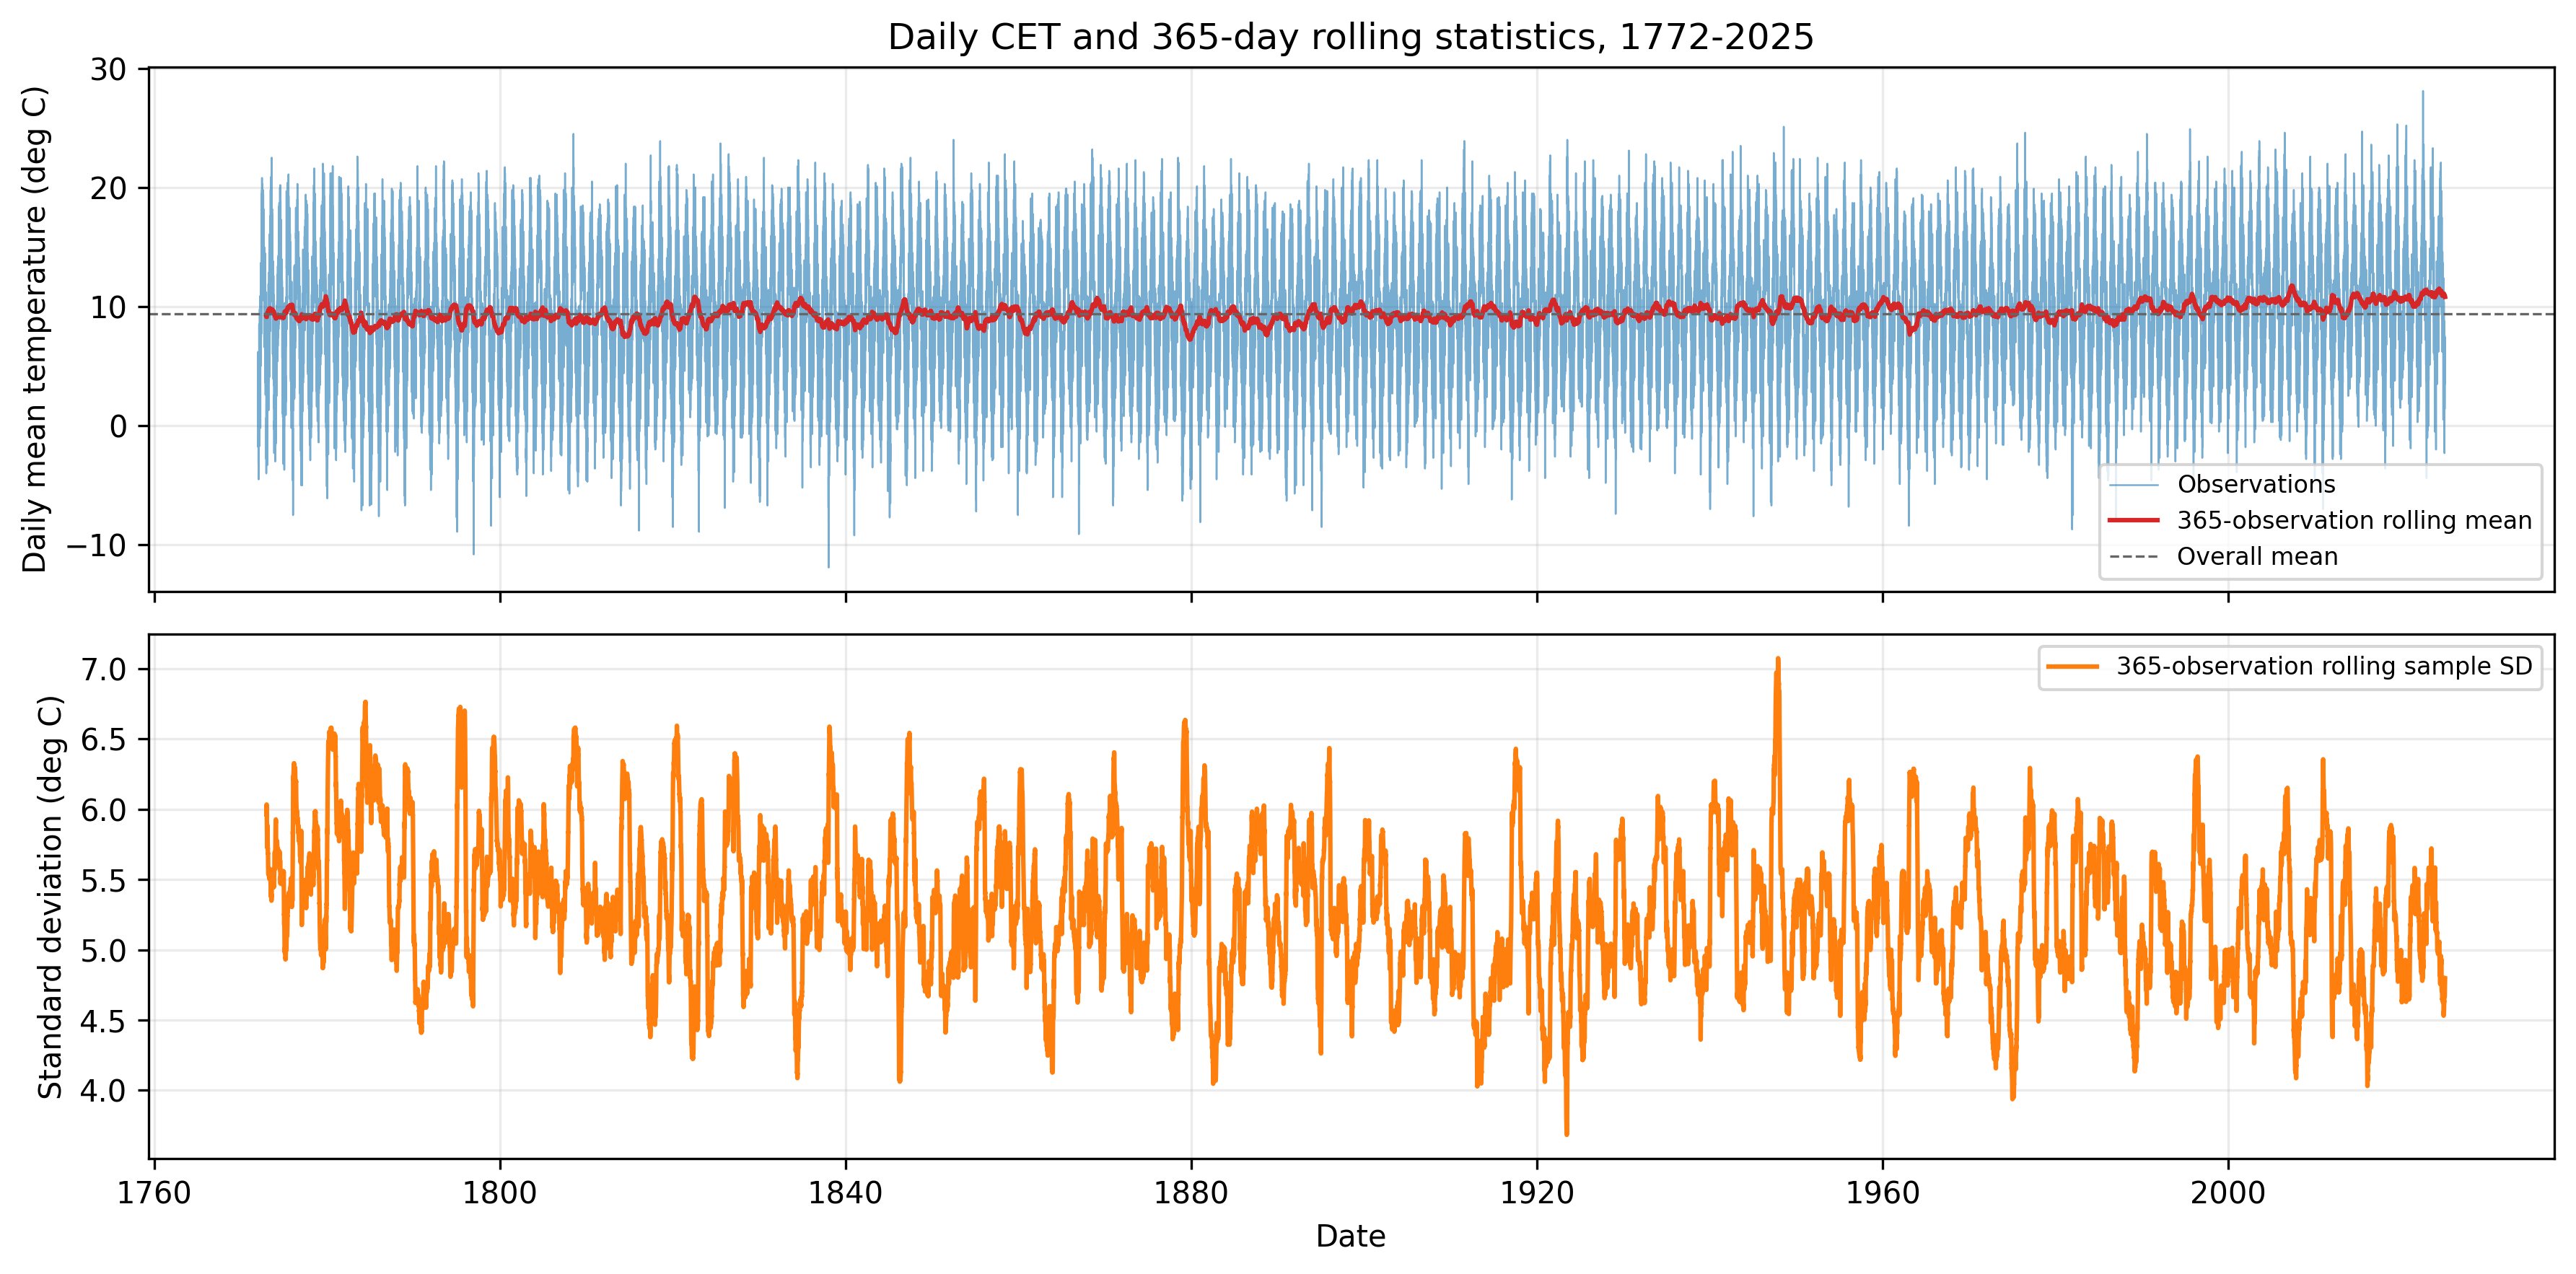
\includegraphics[width=0.9\linewidth]{cet_temp.png}
\end{figure}\par
The raw series does not appear stationary. The displayed summaries use
365-day trailing windows, not monthly averages. They show changes in the long-run
mean, particularly toward the end of the record. Separately, grouping daily
observations by calendar month gives mean temperatures of about $3.48^\circ$C
in January and $16.06^\circ$C in July. Seasonal means and long-run changes are
inconsistent with a constant unconditional mean. Variation in rolling standard
deviations alone is not conclusive evidence of nonstationarity.\par
2. \begin{figure}[htbp]
    \centering
    \graphicspath{{png/}{STATS_Minor/701/HW1/png/}}
    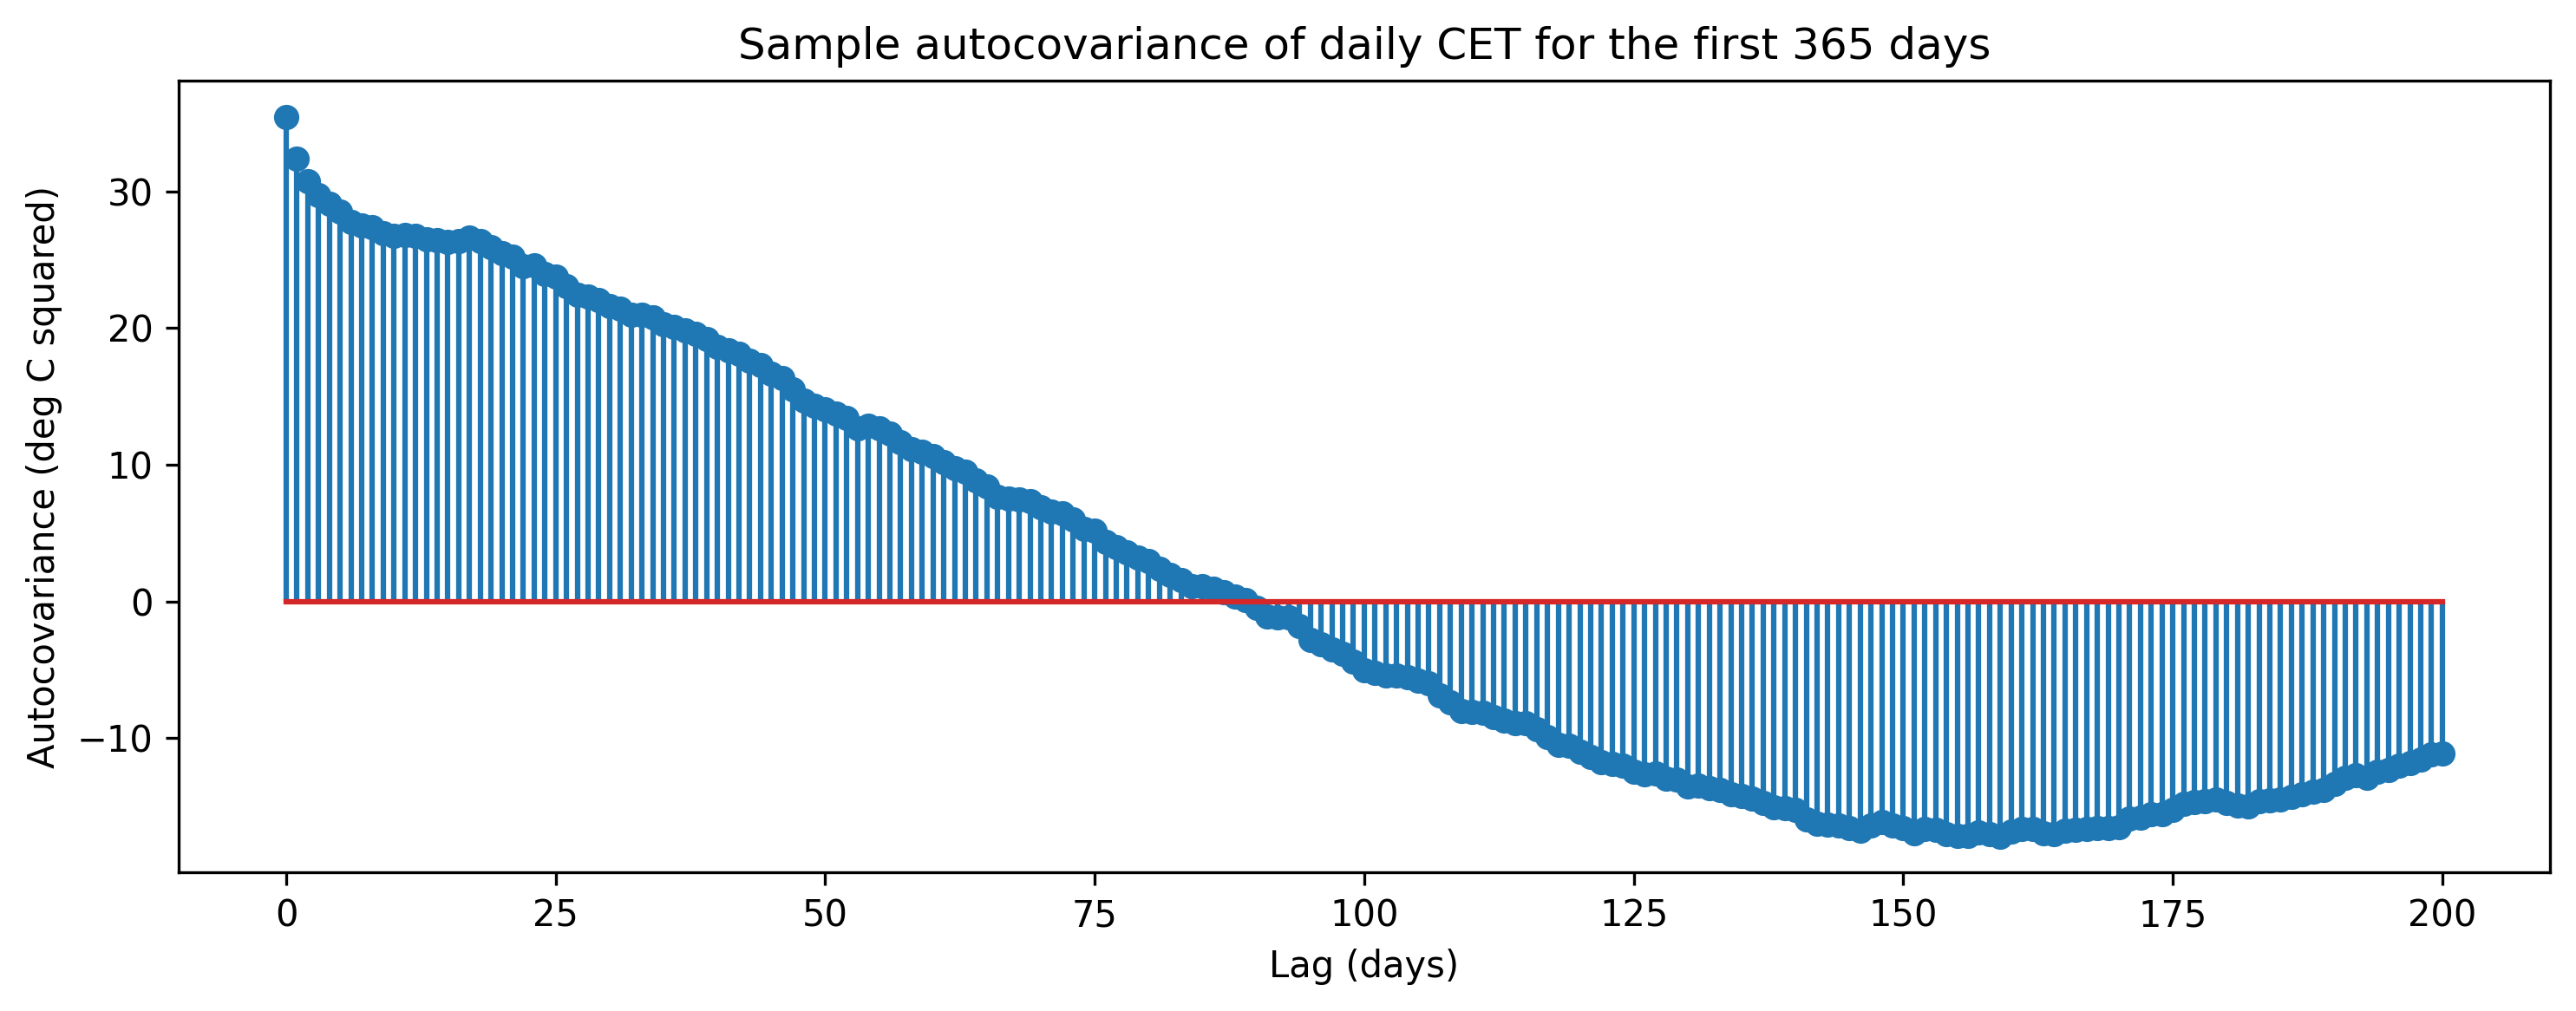
\includegraphics[width=0.8\linewidth]{Lags.png}
\end{figure}\par
Throughout this assignment, ACF denotes the autocovariance function. We use
\[
\widehat\gamma(k)=\frac{1}{n}\sum_{t=1}^{n-k}(x_{t+k}-\bar x)(x_t-\bar x),
\qquad 0\le k<n,
\]
without dividing by $\widehat\gamma(0)$. For these 365 daily observations,
$\widehat\gamma(0)\approx35.47\,{}^\circ\mathrm{C}^2$. The sample autocovariance
crosses zero near lag 90 and reaches a minimum of approximately
$-17.19\,{}^\circ\mathrm{C}^2$ at lag 159, before rising again. This pattern is
consistent with an annual seasonal cycle: nearby observations tend to have
similar deviations from the mean, whereas observations roughly half a year
apart often have deviations of opposite signs. At lag $k$, only $n-k$ pairs
contribute, so large-lag estimates require caution. \par
3. \begin{figure}[htbp]
    \centering
    \graphicspath{{png/}{STATS_Minor/701/HW1/png/}}
    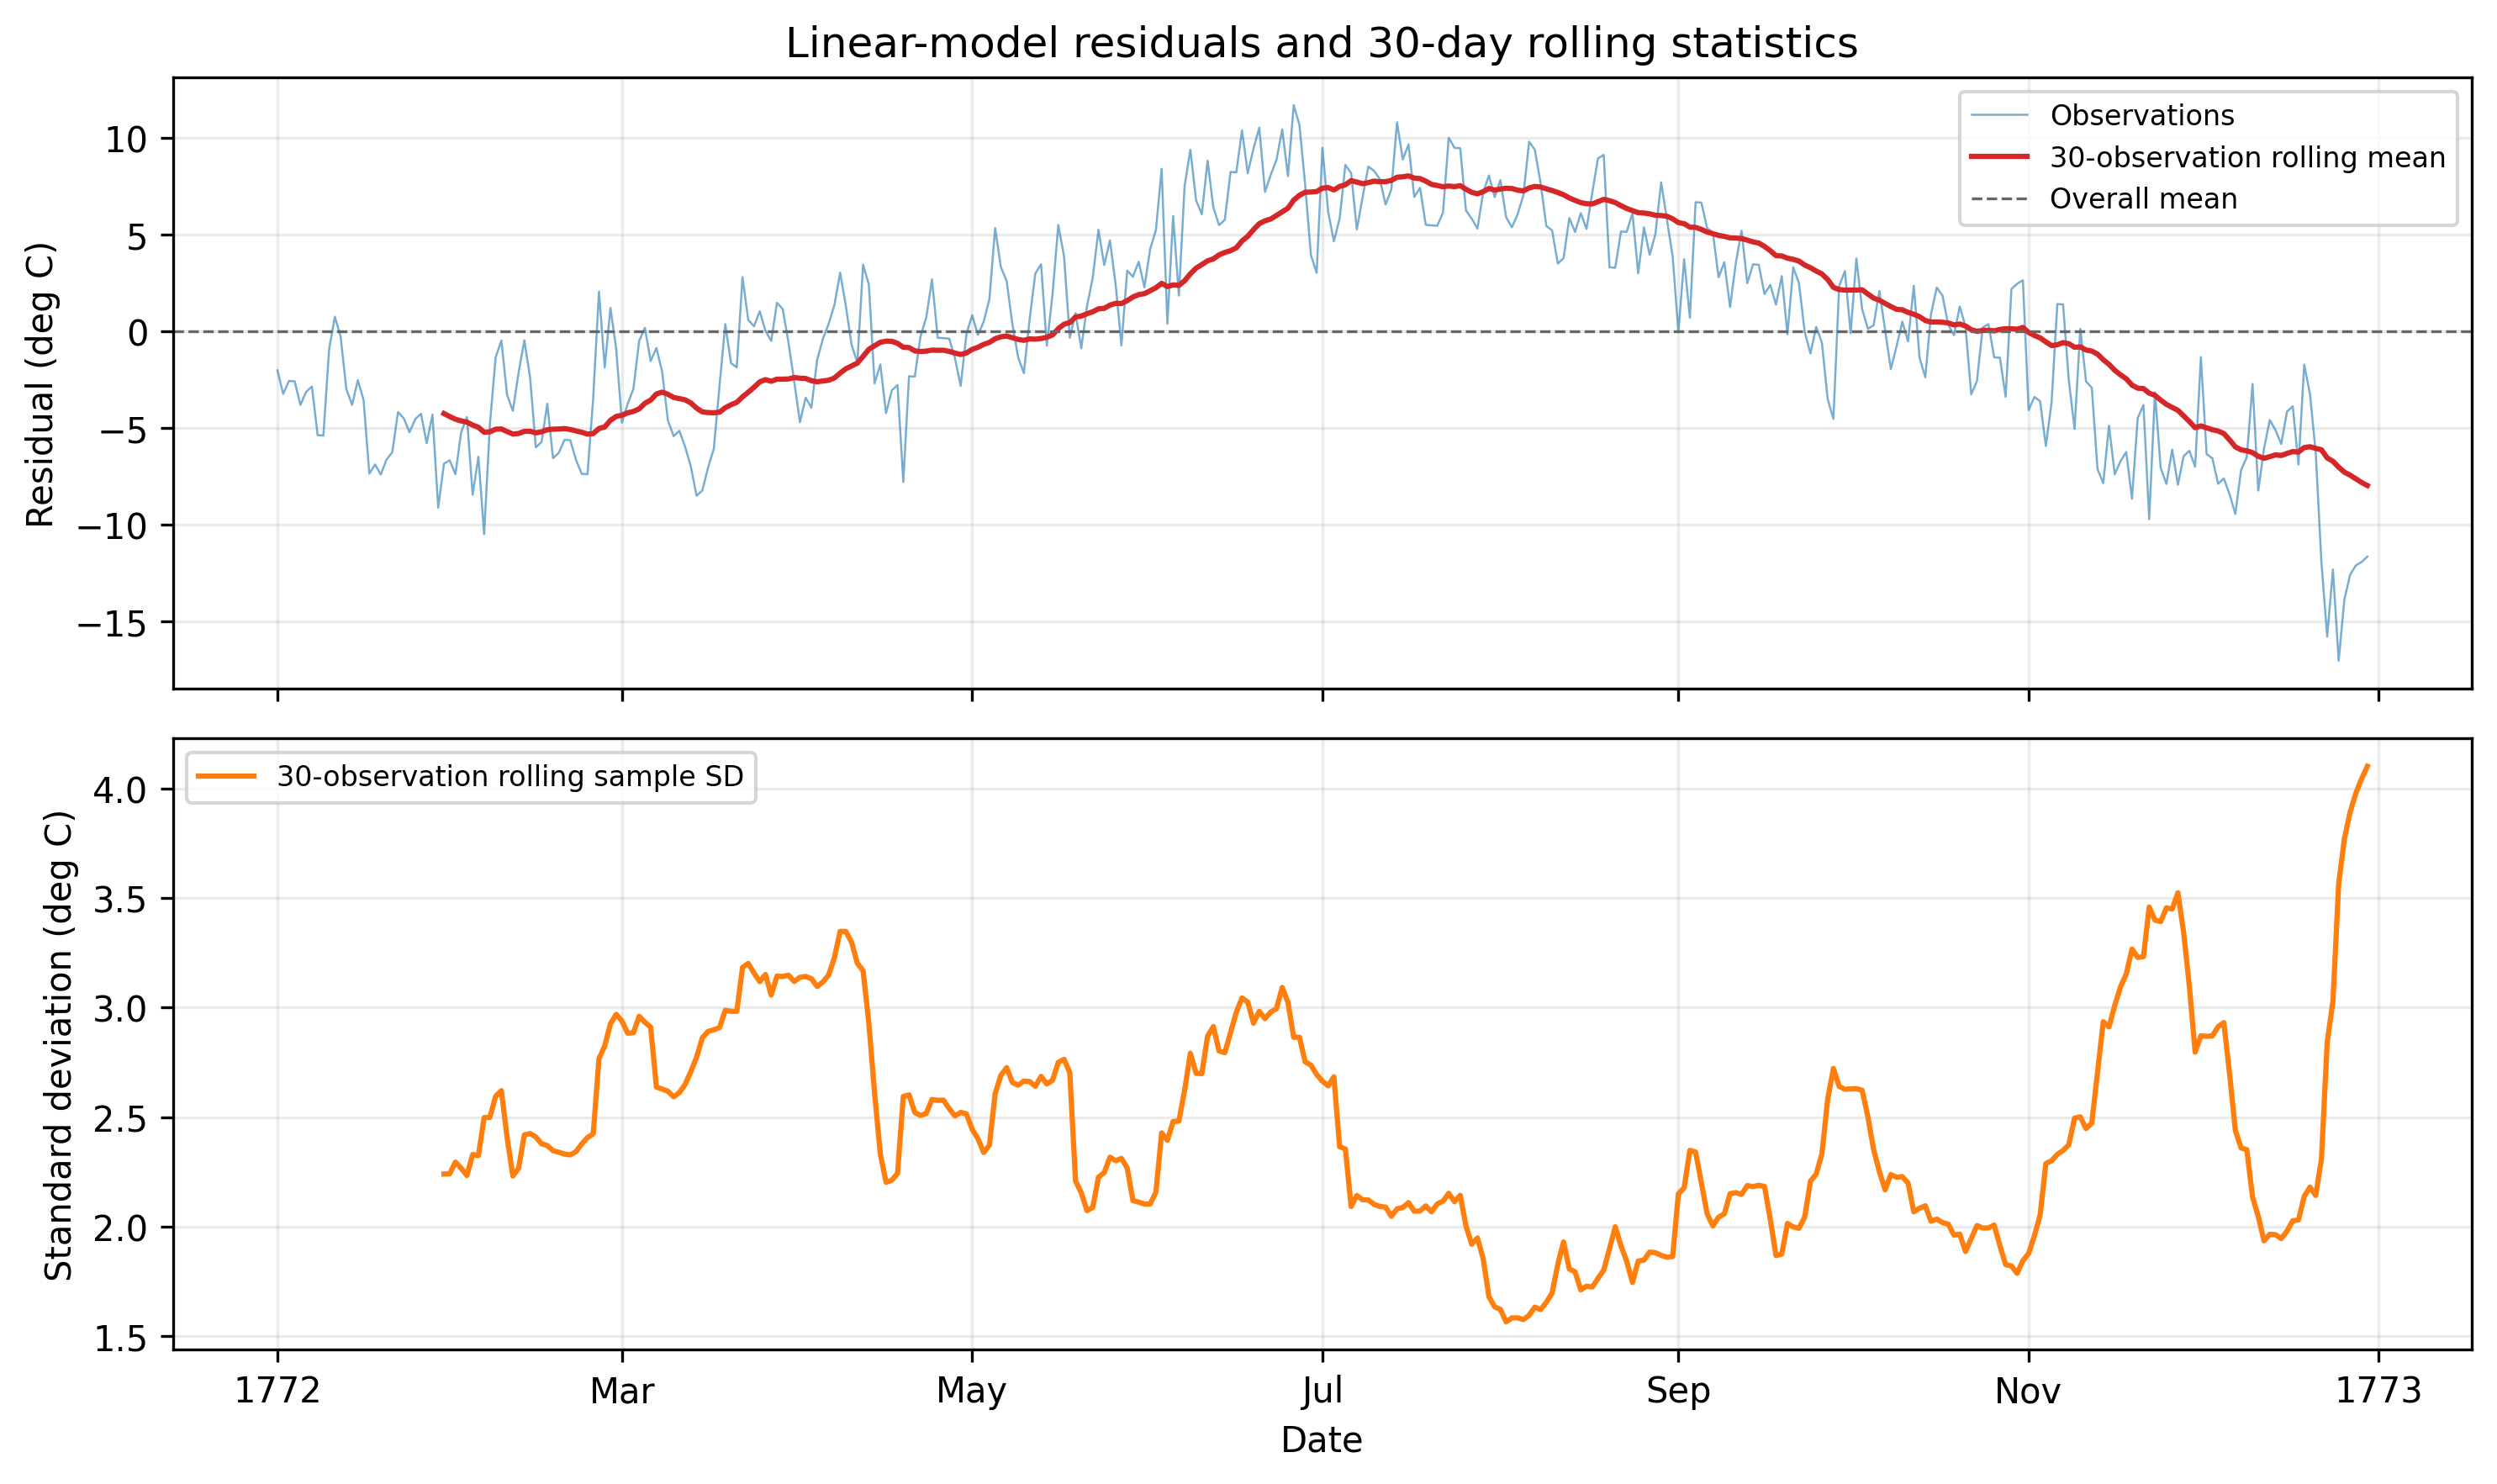
\includegraphics[width=0.8\linewidth]{Residues.png}
\end{figure}\par
The first 365 observations are consecutive daily values starting on
1772-01-01, with no missing values. Using the first-degree specification,
$\widehat m_t=5.1995+0.021813t$. The residuals retain a seasonal shape: negative
near the beginning and end, and positive around the middle. Their 30-day rolling
means range from about $-7.98$ to $8.05^\circ$C. The residual sample
autocovariances at lags $0,1,30,90$ are approximately $30.18,27.02,16.23,-3.04$
in squared degrees Celsius. These broad changes suggest that a straight line
has not removed the seasonal mean. Autocovariance at nonzero lags alone does
not imply nonstationarity, and the residual mean is zero by the OLS normal equations.
\begin{figure}[htbp]\centering
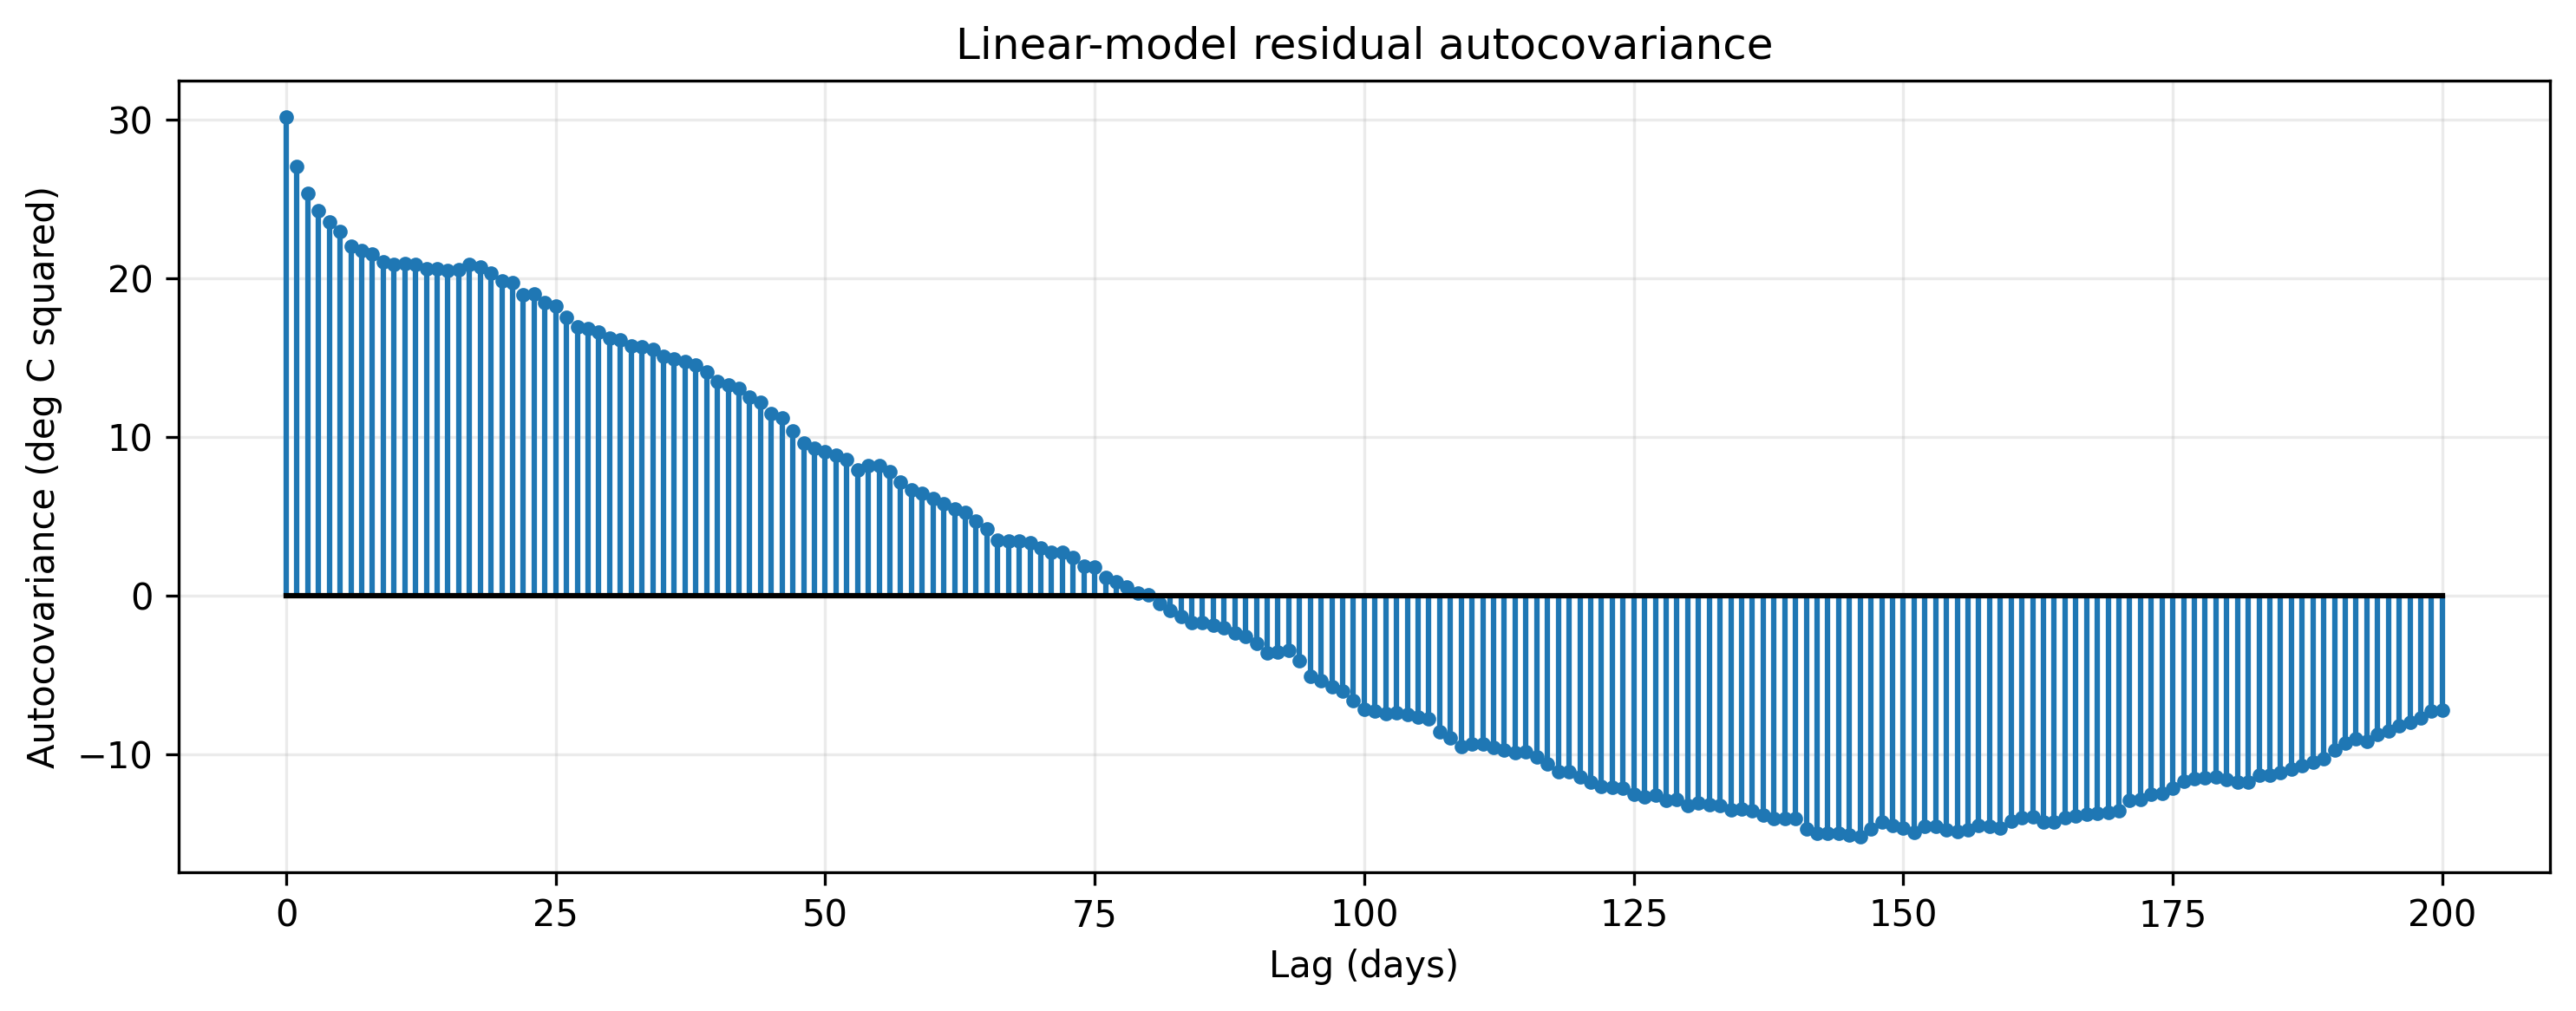
\includegraphics[width=0.8\linewidth]{png/Residual_ACov.png}
\end{figure}\par

4. \begin{figure}[htbp]
    \centering
    \graphicspath{{png/}{STATS_Minor/701/HW1/png/}}
    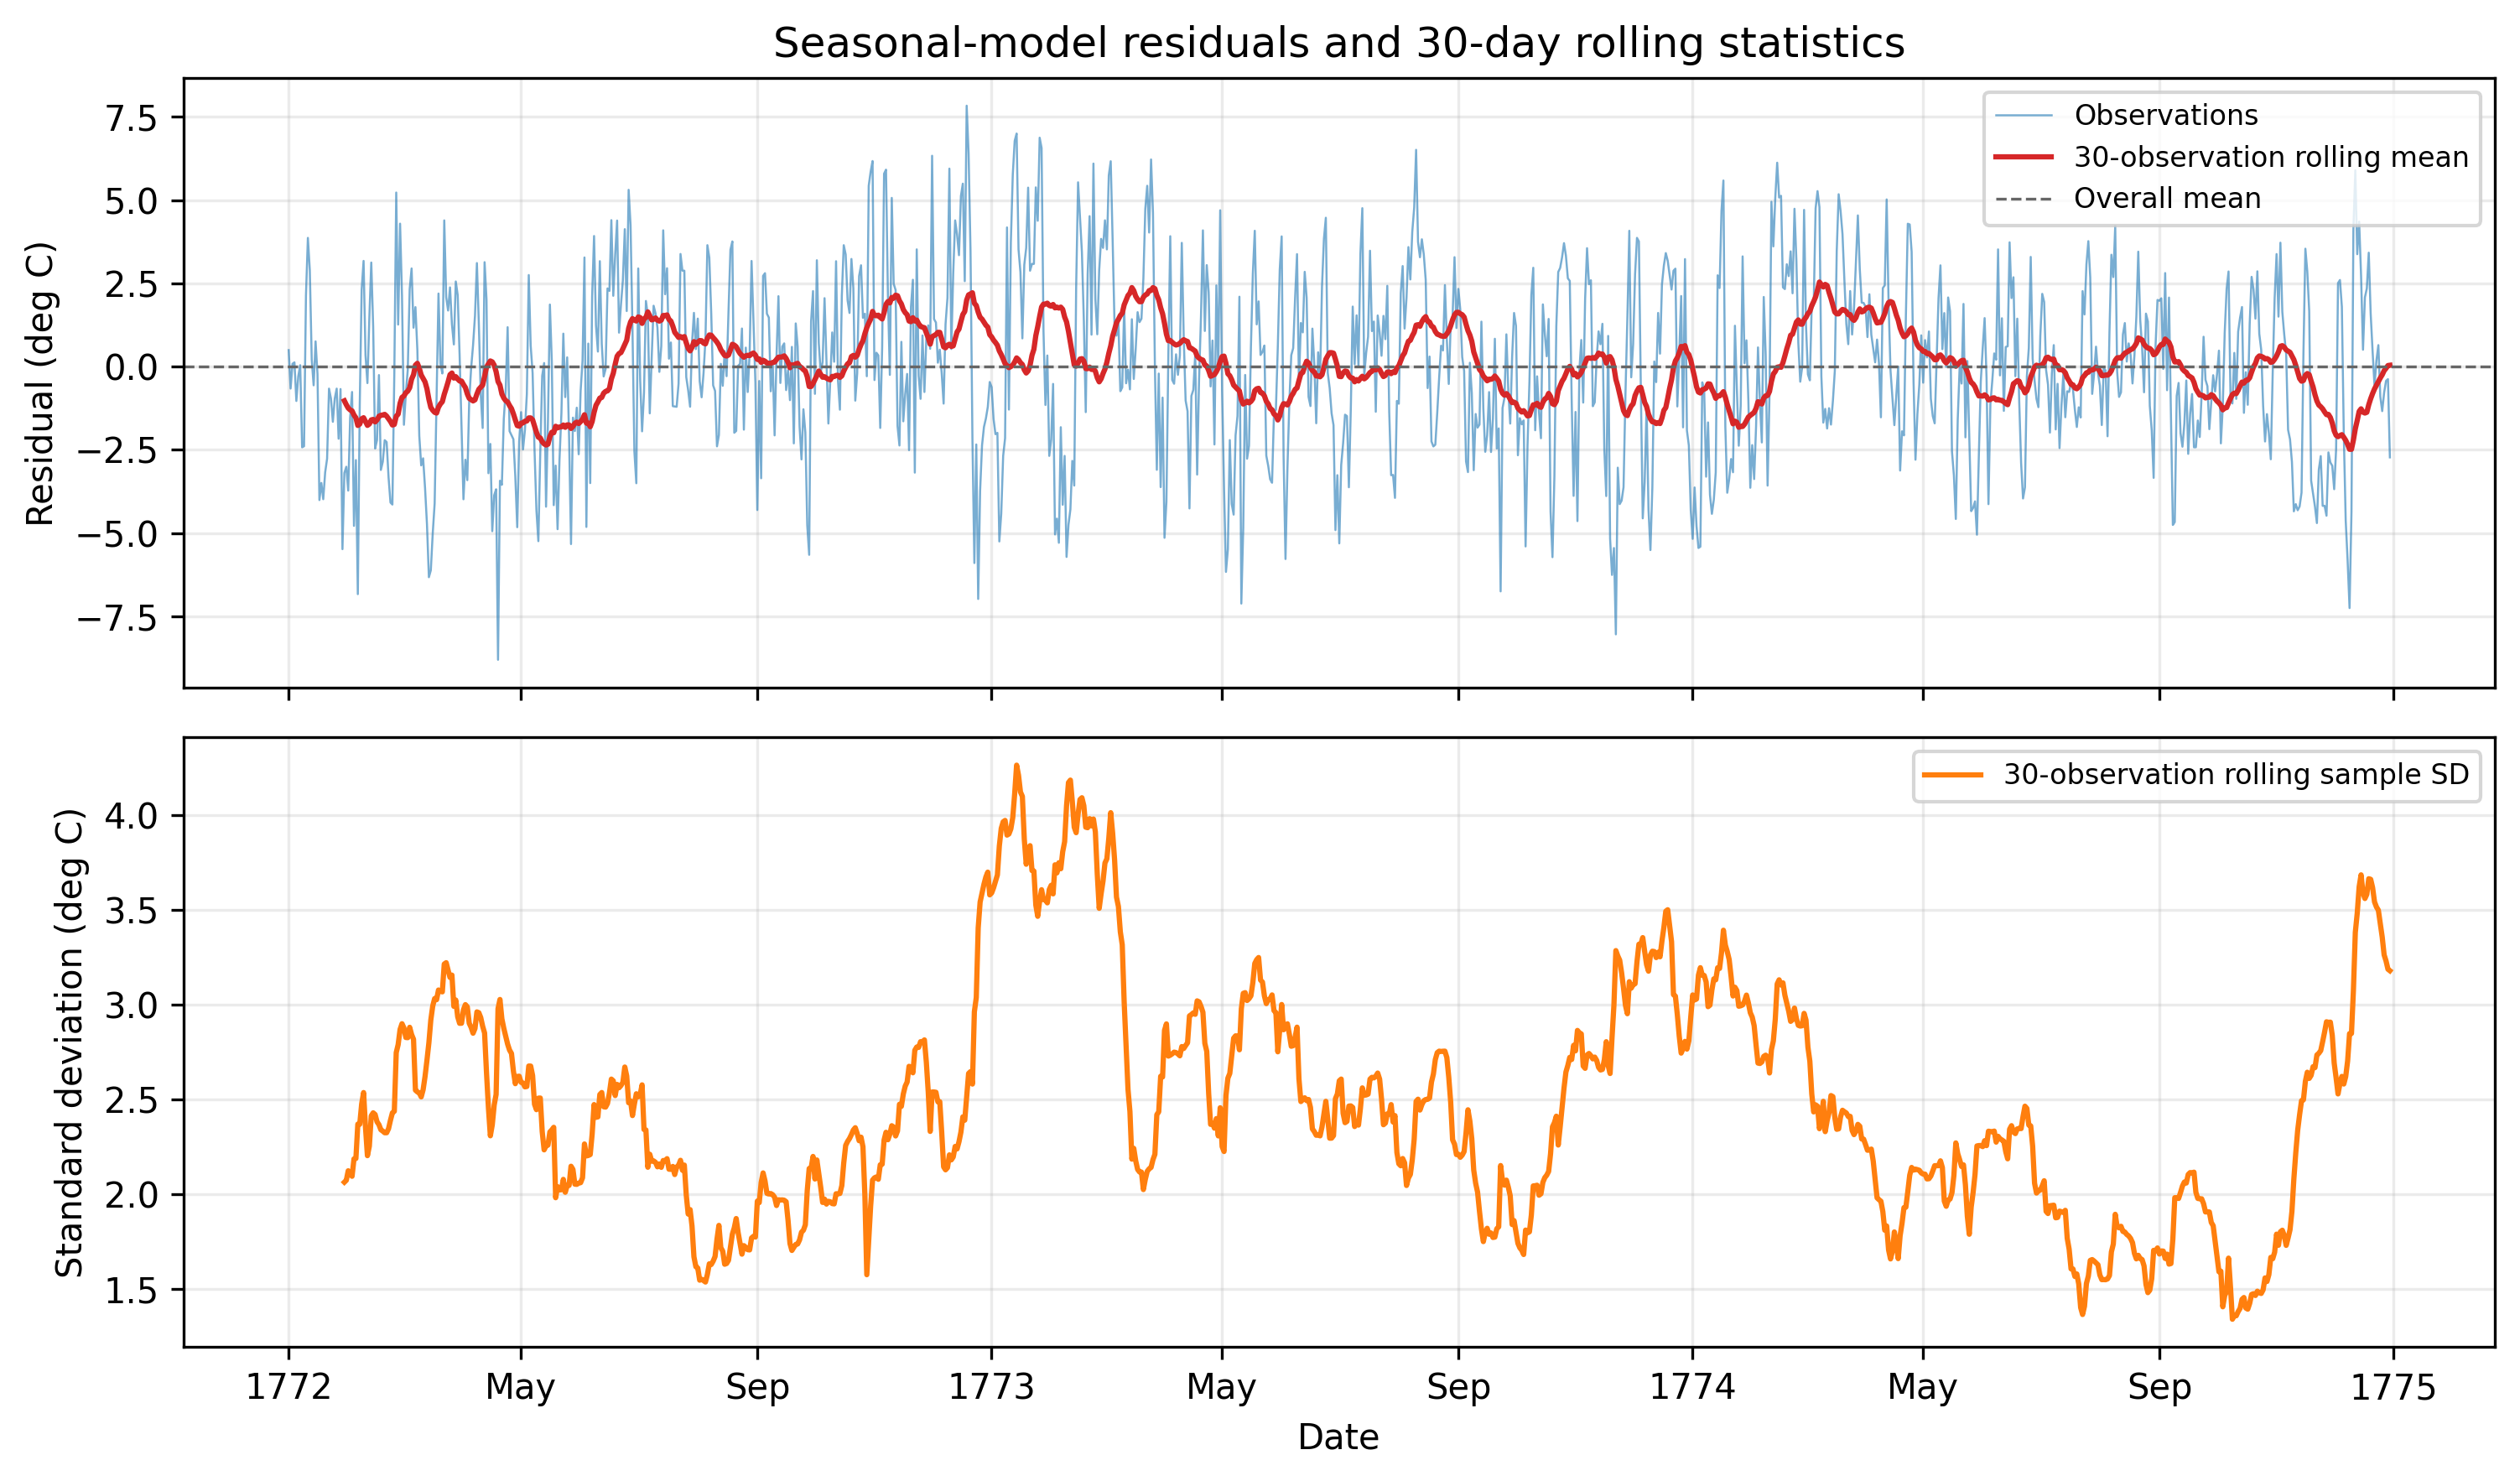
\includegraphics[width=0.8\linewidth]{Tri_Residues.png}
\end{figure}\par
For the first 1095 observations, the fitted mean is
\[
\widehat m_t=9.2522-0.000116t-6.4981\cos(2\pi t/365)-2.8396\sin(2\pi t/365).
\]
The residual 30-day rolling mean ranges from about $-2.48$ to $2.54^\circ$C,
and the rolling sample standard deviation ranges from $1.34$ to $4.26^\circ$C.
The sample autocovariances at lags $0,1,30,90$ are approximately
$7.33,4.73,0.15,-0.14$ in squared degrees Celsius. The seasonal mean structure
is substantially reduced, while short-term dependence remains. These plots
are compatible with a closer approximation to stationarity, but do not establish
it; the 30-day variability estimates also fluctuate. The sample length differs
from part 3, so the numerical differences cannot all be attributed to the model.
\begin{figure}[htbp]\centering
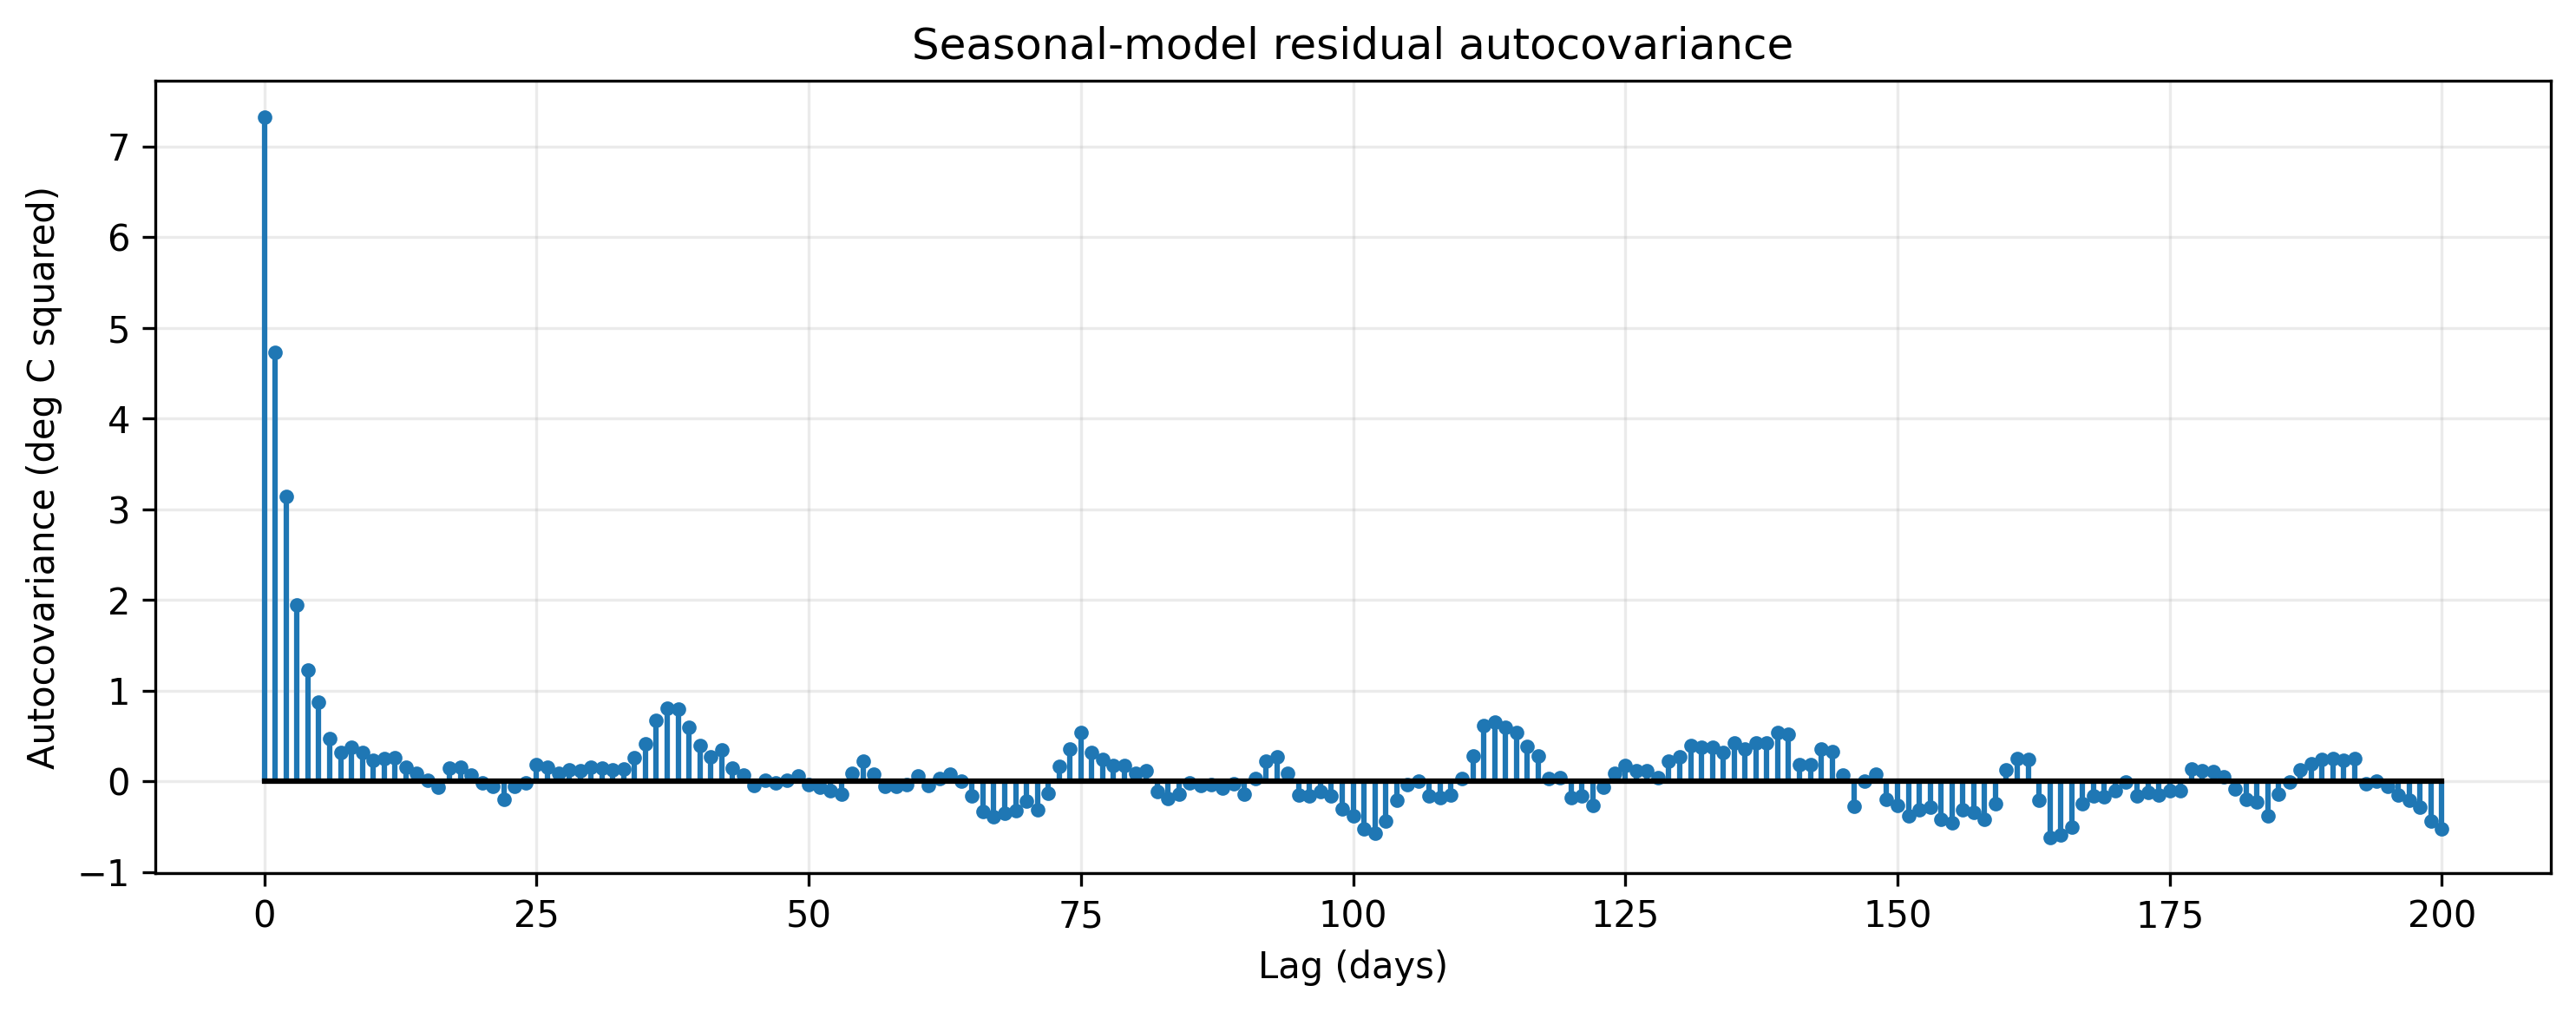
\includegraphics[width=0.8\linewidth]{png/Seasonal_ACov.png}
\end{figure}
For fixed $\omega=2\pi/365$, any phase can be represented through
\[
a\cos(\omega t)+b\sin(\omega t)=R\cos(\omega t-\phi),\quad
R=\sqrt{a^2+b^2},\quad \phi=\operatorname{atan2}(b,a).
\]
Thus $a,b$ are estimated by ordinary linear least squares. Only the frequency
is fixed in advance; if it were unknown, estimating it would generally require
a nonlinear search. When $R=0$, the phase is immaterial.
\par 
\vspace{0.5em}

\subsection*{Problem 8. Trigonometric expansions}

\begin{enumerate}[label=\alph*.]
    \item
    Let $Z_1$ and $Z_2$ be i.i.d. $\mathcal{N}(0,1)$ variables, and
    let $\omega\in[-\pi,\pi)$ be a constant. Define the process
    \[
    Y_t=Z_1\cos(\omega t)+Z_2\sin(\omega t).
    \]
    Calculate its ACF. Is it stationary? Is it strictly stationary?

    \item
    Pick $n$ to be your favorite even integer, say $512$ (although
    $1024$ is also a very good even integer). Set
    \[
    \omega_j=\frac{2\pi j}{n},
    \qquad j=0,1,\ldots,n/2,
    \]
    and simulate $(n/2+1)$ time series of length $n$ given by
    \begin{align*}
    X_{0t}
      &=Z_0,
      & Z_0&\sim\mathcal{N}(0,1),\\
    X_{jt}
      &=Z_{j1}\cos(\omega_jt)+Z_{j2}\sin(\omega_jt),
      & Z_{j1},Z_{j2}&\sim\mathcal{N}(0,2),
      \quad 1\le j<n/2,\\
    X_{n/2,t}
      &=Z_{n/2}(-1)^t,
      & Z_{n/2}&\sim\mathcal{N}(0,1).
    \end{align*}
    Now define a new process by
    \[
    X_t=n^{-1/2}\sum_{j=0}^{n/2}X_{jt}.
    \]

    \begin{enumerate}[label=\arabic*.]
        \item
        Plot your data side-by-side with a white noise series of $n$
        i.i.d. $\mathcal{N}(0,1)$ variables. What do you see?

        \item
        Derive the ACF for $X_t$.

        \item
        Play around with generalizing to
        \[
        \operatorname{Var}(Z_{j1})
        =\operatorname{Var}(Z_{j2})
        =\sigma_j^2,
        \qquad j\ge1,
        \]
        but otherwise not changing your code. Re-run everything and
        look at the resulting plot of your simulated process. Can you
        describe the effect of different choices for
        $\{\sigma_j^2\}$, for example, how things look if
        $\sigma_j^2$ increases or decreases with $j$?
    \end{enumerate}
\end{enumerate}
\vspace{0.5em}
\textbf{Sol.} \par
a. We know
\[
\begin{aligned}
    \gamma_Y(t,t+h) &= \mathbb{E}(Z_1\cos(\omega t) +Z_2 \sin(\omega t))(Z_1\cos(\omega(t+h)) +Z_2 \sin(\omega(t+h))) \\ &= \cos(\omega t)\cos(\omega(t+h)) + \sin(\omega t)\sin(\omega(t+h)) \\
    &=\cos(\omega h),
\end{aligned} 
\]
which is constant about $t$ and hence $Y_t$ is a stationary process, with autocovariance function
\[
\gamma_Y(h) = \cos(\omega h).
\]
For $\mathbf{t} : =(t_1,\cdots,t_k) \in \Z^k$, we know
\[
\mathbf{Y}_{\mathbf{t}} :=(Y_{t_1},\cdots,Y_{t_k})^T = \begin{bmatrix}
    \cos(\omega t_1) & \sin(\omega t_1) \\
    \vdots & \vdots \\
    \cos(\omega t_k) & \sin(\omega t_k)
\end{bmatrix}\begin{bmatrix}
    Z_1 \\
    Z_2
\end{bmatrix}
\]
and hence $\mathbf{Y}_{\mathbf{t}}$ is a normal random vector with covariance matrix
\[
\begin{bmatrix}
    \cos(\omega t_1) & \sin(\omega t_1) \\
    \vdots & \vdots \\
    \cos(\omega t_k) & \sin(\omega t_k)
\end{bmatrix}\begin{bmatrix}
    \cos(\omega t_1) & \sin(\omega t_1) \\
    \vdots & \vdots \\
    \cos(\omega t_k) & \sin(\omega t_k)
\end{bmatrix}^T = [\cos (\omega(t_i-t_j))]_{i,j = 1} ^k
\]
and hence
\[\mathbf{Y}_{\mathbf{t}} \overset{d}{=} \mathbf{Y}_{\mathbf{t}+h} \]
where $\mathbf{t}+h:=(t_1+h,\cdots,t_k+h)$ for any $h\in\Z$ because they are Gaussian vectors with the same zero mean and covariance matrix. Therefore, $Y_t$ is strictly stationary as well.\par
b. 1. We compare the simulated series with an independently generated
$N(0,1)$ white-noise sample. Both show irregular zero-centered fluctuations of
similar size, with sample autocovariances near zero away from lag zero.
For $n$ consecutive observations the simulated Gaussian vector has covariance
$I_n$, so it has exactly the same distribution as $n$ independent standard normals.
The infinite extension is periodic, $X_{t+n}=X_t$, and is not white noise at all lags.
\begin{figure}[htbp]
    \centering
    \graphicspath{{png/}{STATS_Minor/701/HW1/png/}}
    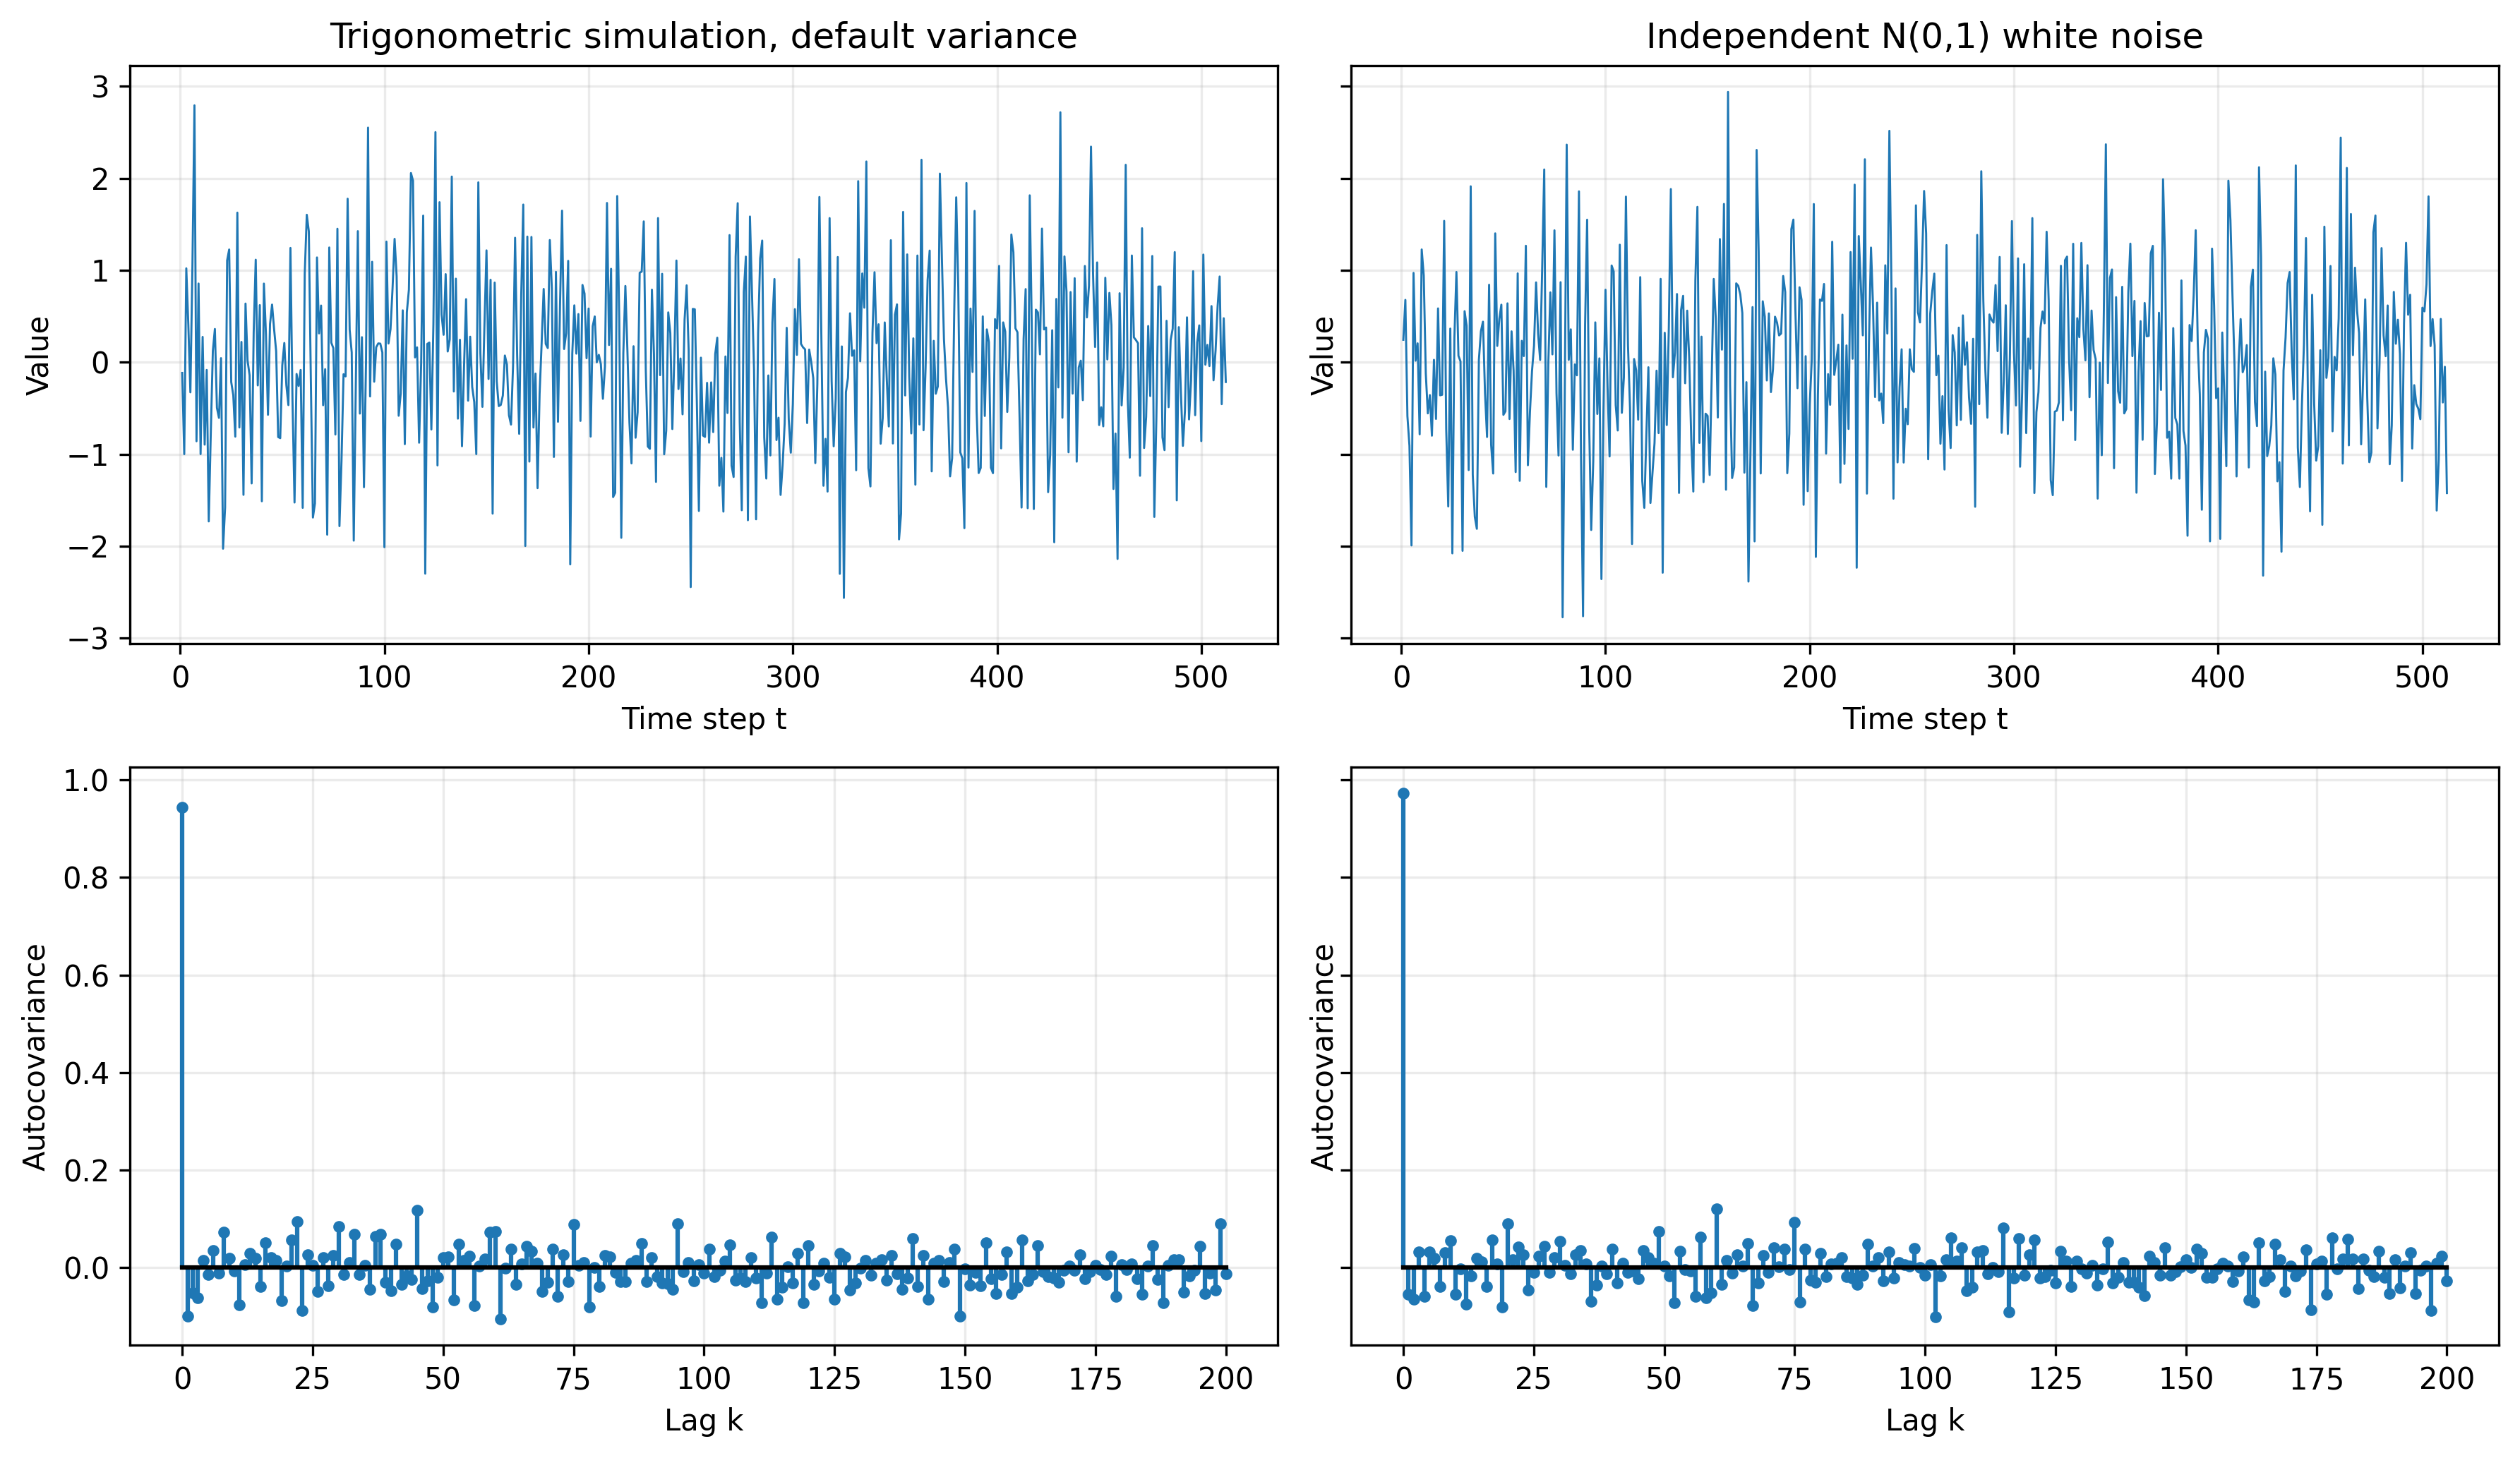
\includegraphics[width=0.8\linewidth]{HW1_5_default.png}
\end{figure}
\par
2. We may write $X_t$ explicitly as
\[
X_t = \dfrac{1}{\sqrt{n}}\left(Z_0 + \sum\limits_{j=1}^{n/2-1}(Z_{j1}\cos(\omega_jt)+Z_{j2}\sin(\omega_jt)) + Z_{n/2}(-1)^t\right)
\]
and then
\[
\begin{aligned}
\gamma_X(t,t+h)
&=\frac{1}{n}\left[1+(-1)^h+2\sum_{j=1}^{n/2-1}\cos\left(\frac{2\pi jh}{n}\right)\right]\\
&=\begin{cases}
1,&h\in n\mathbb{Z},\\
0,&h\notin n\mathbb{Z}.
\end{cases}
\end{aligned}
\]
\par
3. For $j=1,\ldots,255$, define $u_j=(j-1)/254$. We compare
\[
    \sigma_j=0.1+4.9u_j
    \quad\text{and}\quad
    \sigma_j=0.1+\frac{4.9}{2}\bigl(1-\cos(6\pi u_j)\bigr).
\]
In both cases, $\operatorname{Var}(Z_{j1})=\operatorname{Var}(Z_{j2})=\sigma_j^2$;
the endpoint coefficients retain variance 1. The first choice increases linearly
with frequency, whereas the second oscillates across frequency bands.
Increasing $\sigma_j$ emphasizes rapid oscillations and tends to produce
negative short-lag covariance; decreasing weights would emphasize low frequencies
and smoother variation. Oscillating weights emphasize selected frequency bands,
creating a different lag-dependence pattern. The index $j$ is frequency, not time:
these weights do not make the variance increase with $t$. In fact,
\[
\gamma_X(h)=\frac1n\left[1+(-1)^h+
\sum_{j=1}^{n/2-1}\sigma_j^2\cos(2\pi jh/n)\right],
\]
Both constructions are stationary Gaussian processes. Their covariance is
generally nonzero at some nonzero lags.
\begin{figure}[htbp]
    \centering
    \graphicspath{{png/}{STATS_Minor/701/HW1/png/}}
    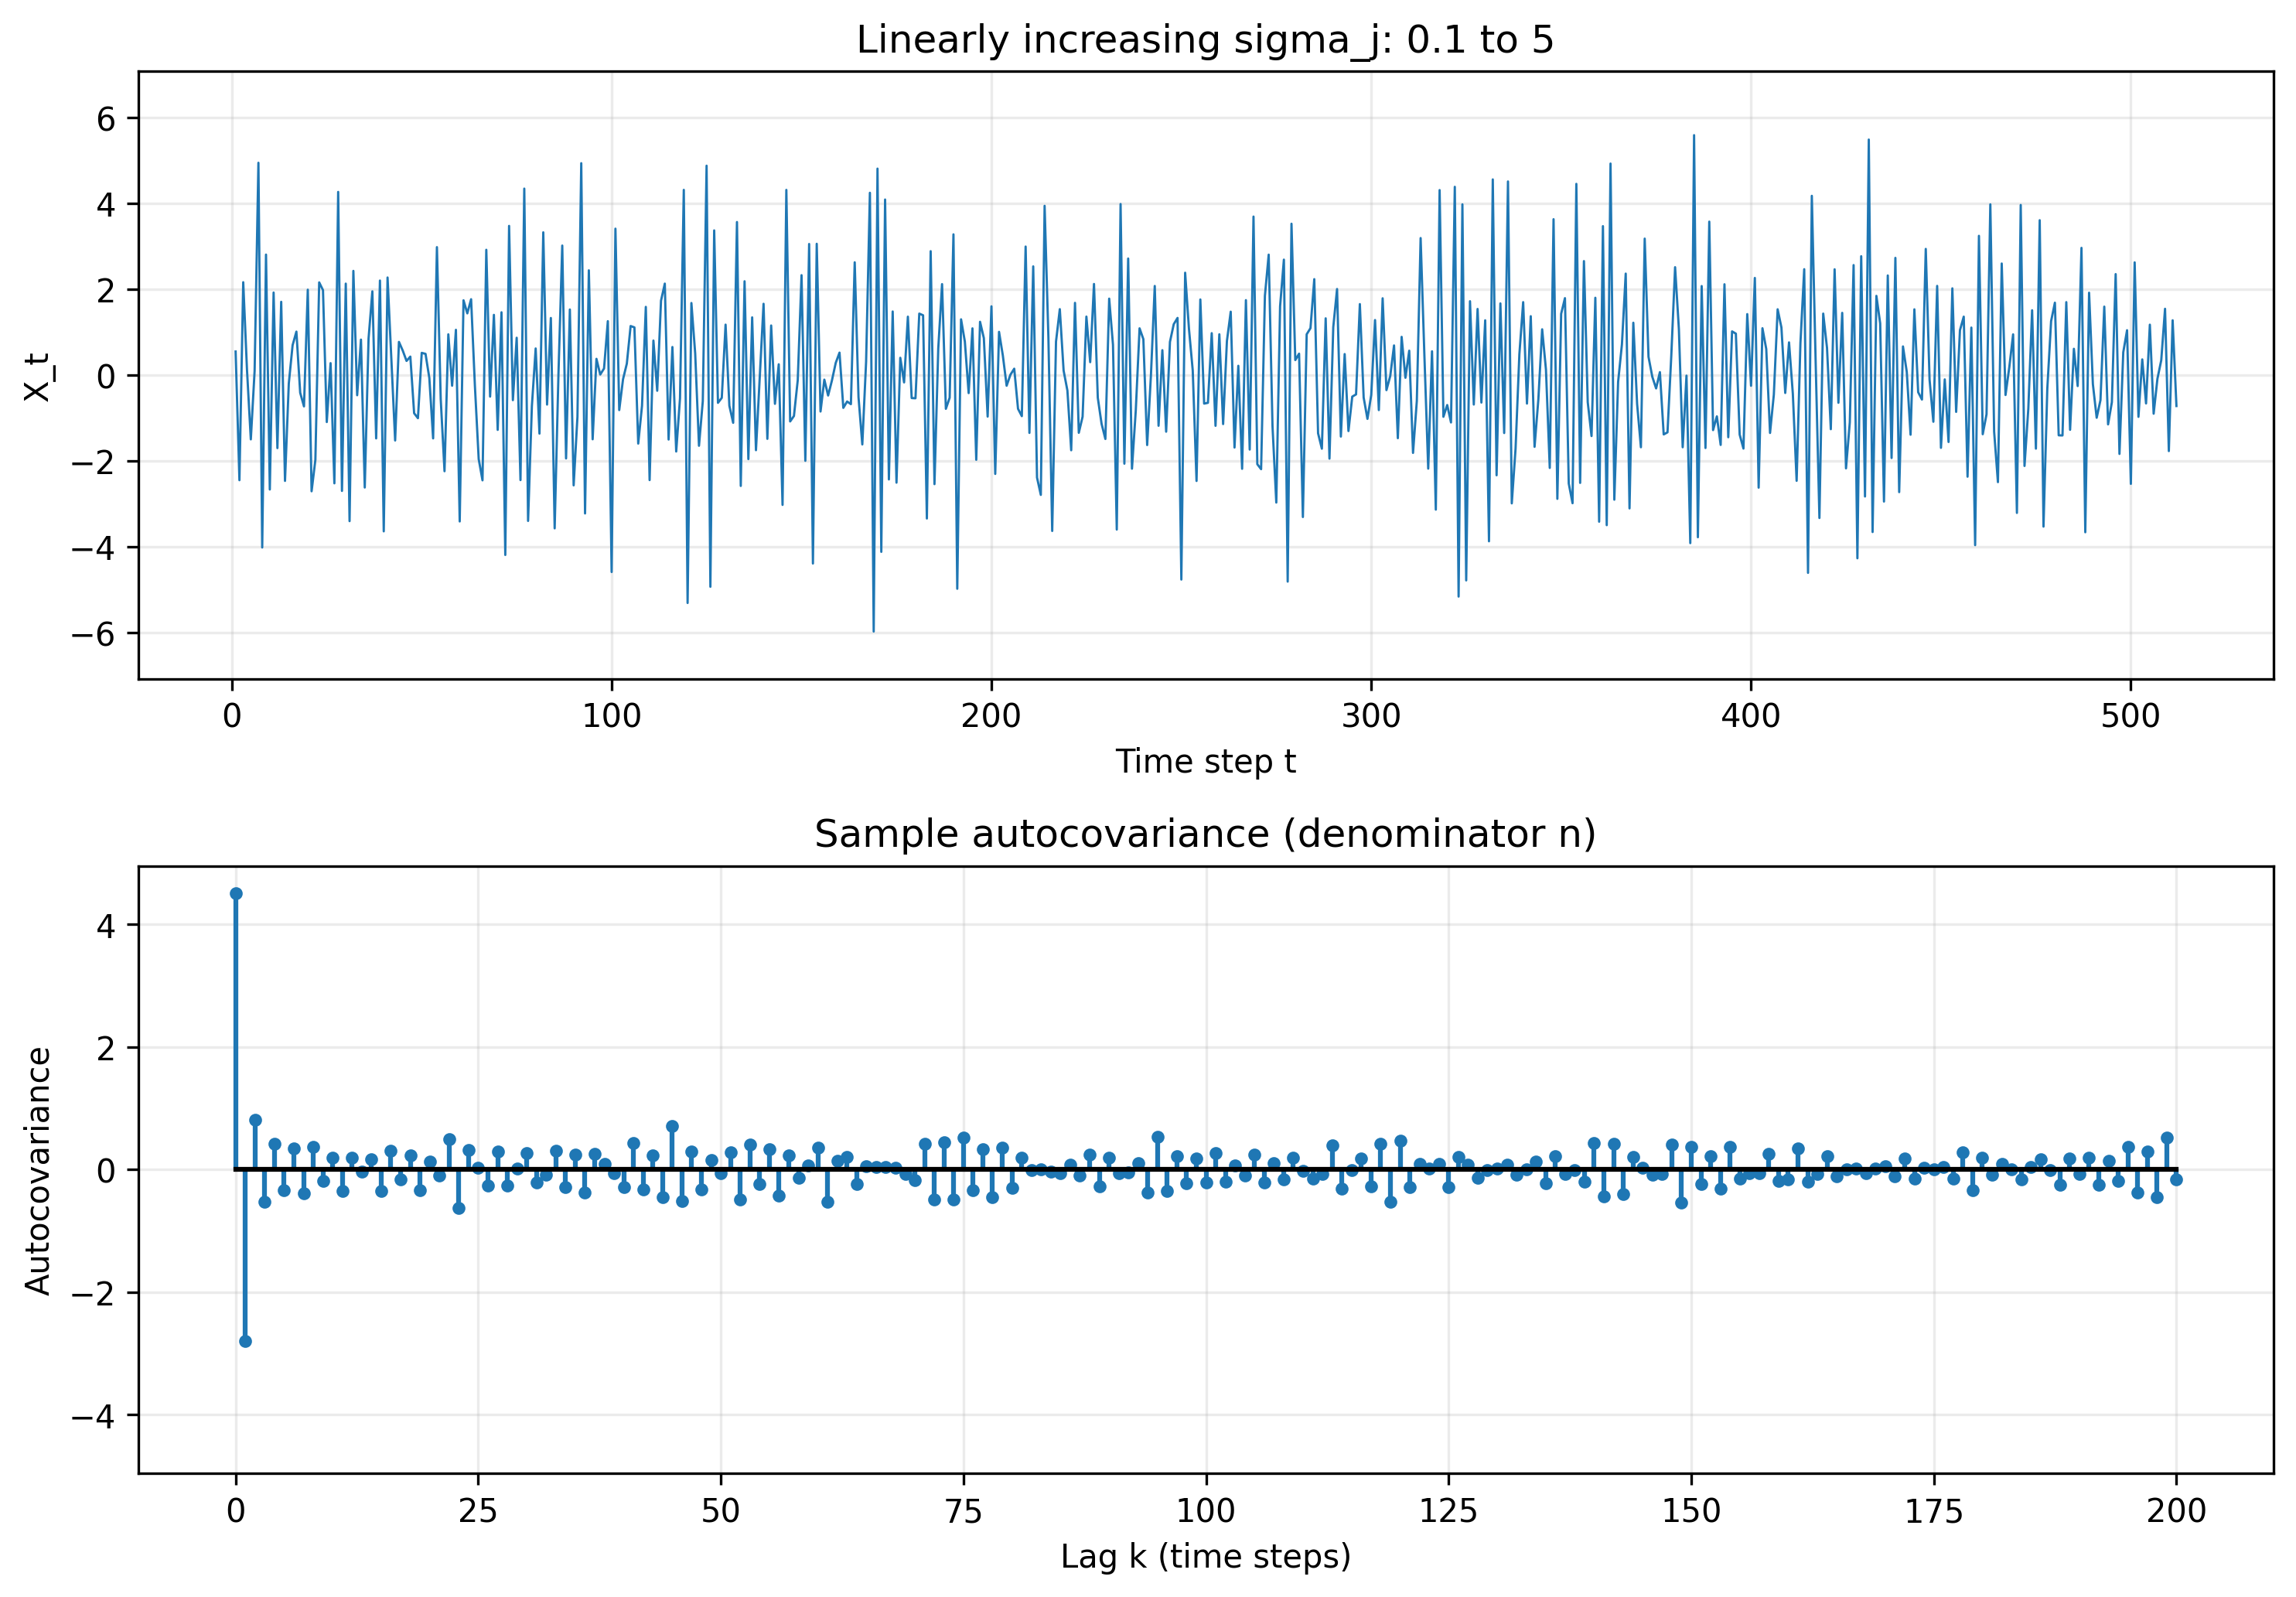
\includegraphics[width=0.8\linewidth]{HW1_5_sigma_linear.png}
\end{figure}
\begin{figure}[htbp]
    \centering
    \graphicspath{{png/}{STATS_Minor/701/HW1/png/}}
    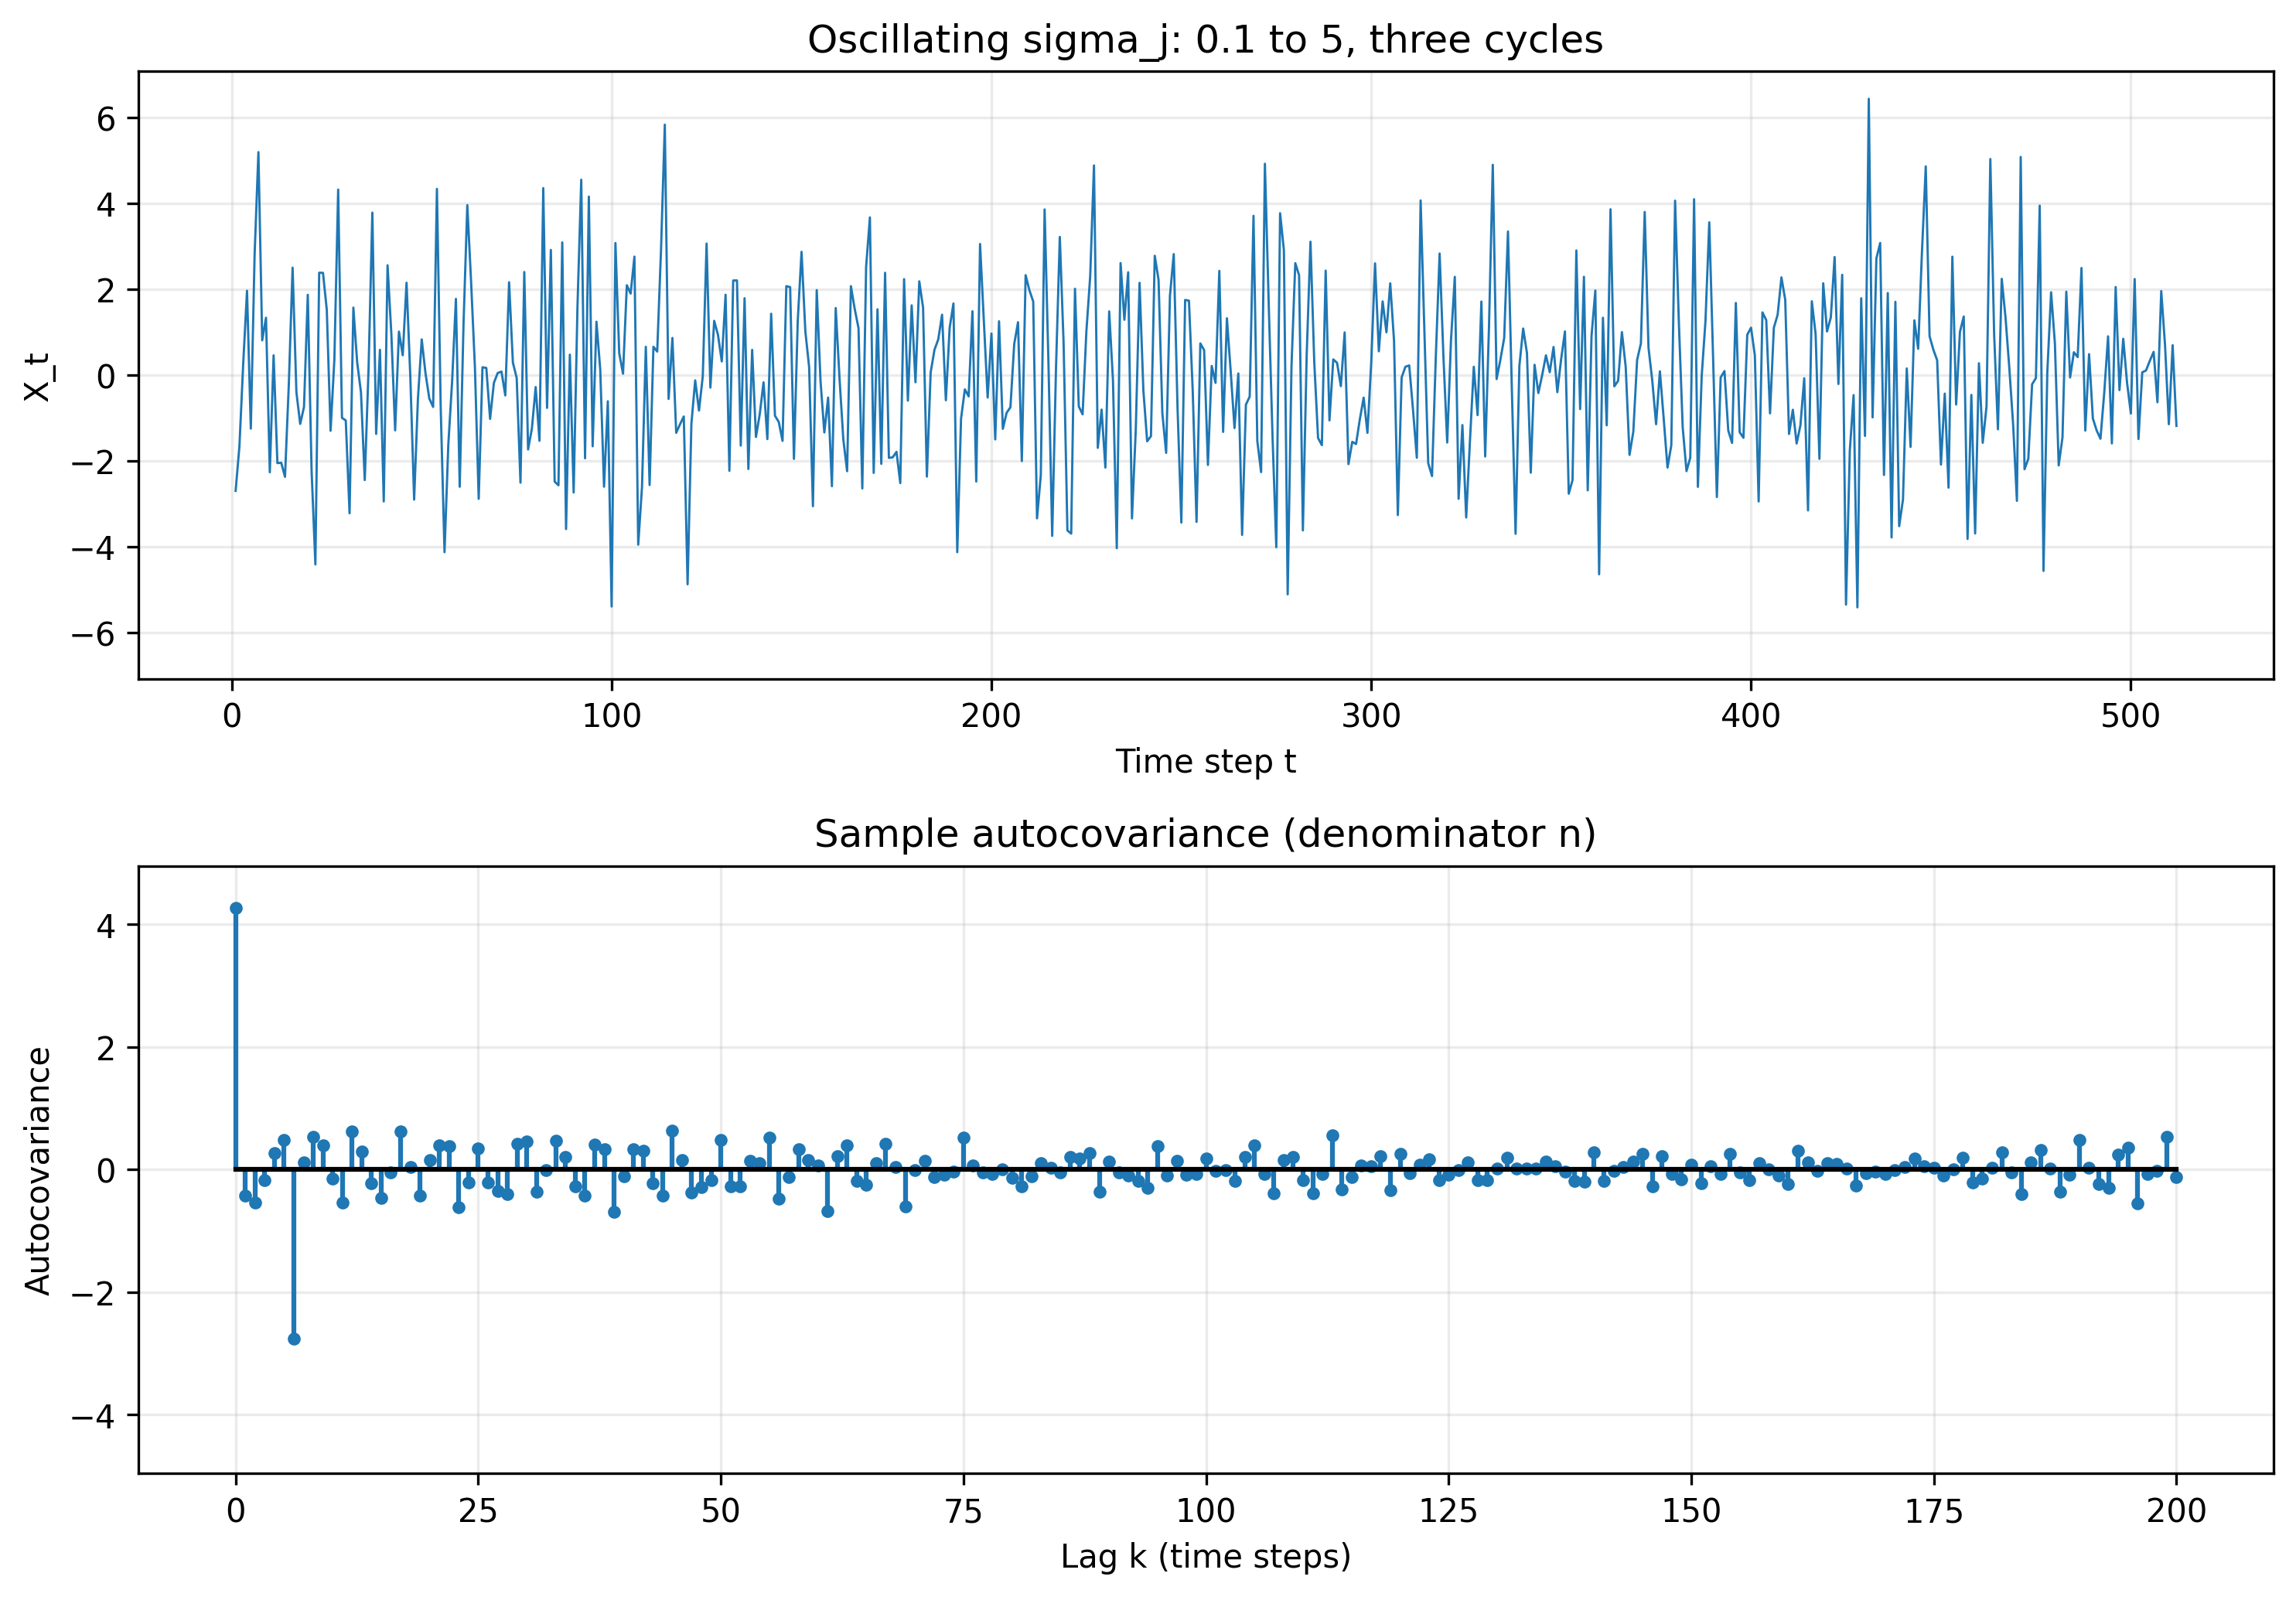
\includegraphics[width=0.8\linewidth]{HW1_5_sigma_oscillating.png}
\end{figure}\par

\vspace{0.5em}

\clearpage
\appendix
\section{Python code}
The scripts read \texttt{code/cet.csv} relative to their own location and save
figures in \texttt{png/}. ACF uses the denominator $n$ without variance normalization.
\subsection{Sample autocovariance}
\lstinputlisting[language=Python]{code/autocovariance.py}
\subsection{CET data analysis}
\lstinputlisting[language=Python]{code/HW1_4.py}
\clearpage
\subsection{Gaussian trigonometric simulations}
\lstinputlisting[language=Python]{code/HW1_5.py}

\end{document}
